% Copyright (C) 2018 by latexstudio <http://www.latexstudio.net>
%
% This program is free software: you can redistribute it and/or modify
% it under the terms of the GNU General Public License as published by
% the Free Software Foundation, either version 3 of the License, or
% (at your option) any later version.
%
% This program is distributed in the hope that it will be useful,
% but WITHOUT ANY WARRANTY; without even the implied warranty of
% MERCHANTABILITY or FITNESS FOR A PARTICULAR PURPOSE.  See the
% GNU General Public License for more details.
%
% You should have received a copy of the GNU General Public License
% along with this program.  If not, see <http://www.gnu.org/licenses/>.
%

%\documentclass{ctexart}
%
%\setCJKmainfont{Source Han Sans SC}
%  %[
%  %  UprightFont    = * Medium,
%  %  BoldFont       = * Bold,
%  %  ItalicFont     = * Medium,
%  %  BoldItalicFont = * Bold
%  %]
%\begin{document}
%你好,世界
%
%\end{document}

\documentclass{latex-faq-cn-class}
% 如果遇到字体问题,可以选择不使用自定义字体:
% \documentclass[use-customized-fonts=false]{latex-faq-cn-class}

\usepackage{dirtree}

% TODO: 移植到 class
% \makeatletter
% \def\@captype{figure}
% \makeatother

\title{\LaTeX{} 常见问题}
\author{\LaTeX{} Studio 团队}

\begin{document}

\maketitle

% \def\FONTTEST{字体测试骨头 ABC fi fl\ }
% \FONTTEST \textit{\FONTTEST} \textbf{\FONTTEST \textit{\FONTTEST}}          \par
% \textsf{\FONTTEST \textit{\FONTTEST} \textbf{\FONTTEST \textit{\FONTTEST}}} \par
% \texttt{\FONTTEST \textit{\FONTTEST} \textbf{\FONTTEST \textit{\FONTTEST}}}

\section{日经问题}
\label{sec:starter}

这里是一些几乎每天都会被提及的问题,但有些其实并不是真正的问题。它们往往是指向后面问题的链接。

\begin{faq}{论文 / 比赛的 deadline 要到了,如何在一天 / 两天 / 三天之内入门 \LaTeX{}?}[get-started]
  非常遗憾,这几乎是不可能完成的任务。在时间紧张、压力巨大的情形下,入门 \LaTeX{} 对您来说没有意义。
  作为排版工具,\LaTeX{} 实现的效果远没有文章的内容重要,所以请不要在这种情况下把您的精力投入在学习
  \LaTeX{} 上。
  
  通常来说,我们建议您至少通过三个月的时间来入门 \LaTeX{},并在之后的工作、学习中不断深入理解、
  积累经验。
  
  如果确有必要在短时间内掌握 \LaTeX{} 的使用方法,请联系靠谱且有经验的人。注:很多“学长”、“老师”都是
  不靠谱的,所以这一点实际上很难办到。
\end{faq}

\begin{faq}{如何“安装 \LaTeX{}”?}[install-latex]
  如果您也有这一问题,首先需要澄清一些概念,见~\ref{}。简短来说,\LaTeX{} 本身是一种标记语言,而非
  Microsoft Word 一样现成的软件。因此,社区将相关的支持文件、可执行程序、文档等打包在一起,形成了可供
  用户下载、安装的发行版(distribution)。一般而言,“安装 \LaTeX{}”指的就是安装发行版。
  
  目前,根据平台不同,可供使用的主流发行版有以下这些:
  
  \begin{itemize}
  
    \item \TeXLive{},见~\faqref{install-texlive}
    \item \MiKTeX{},见~\faqref{install-miktex}
    \item \MacTeX{},适用于 macOS,见~\faqref{install-mactex}
    % TODO: 更多的发行版介绍
    \item 【有待整理】
  \end{itemize}
\end{faq}

\begin{faq}{我的 \CTeX{} 为什么……}[why-ctex]
  您在这里提到的“\CTeX{}”,指的很可能是由中国 \TeX{} 社区(即 \CTeX{} 社区)所发布的、以 \MiKTeX{}
  为基础的一个发行版,全称为“\href{http://www.ctex.org/CTeX}{\CTeX{} 套装}”。这一发行版目前已停止
  维护,所以除非必要,请不要再使用。\TeXLive{} 以及 \MiKTeX{} 都是可靠的替代方案。
  
  \CTeX{} 社区另发布了一个同样称为 \href{https://www.ctan.org/pkg/ctex}{\CTeX{} 的宏集}(宏包),
  这是目前在 \LaTeX{} 中使用中文排版的推荐方案。如果您需要获取相关信息,请查阅其文档。\CTeX{} 宏集
  的有关问题,在本文之后也有涉及。
\end{faq}

% Copyright (C) 2018 by latexstudio <http://www.latexstudio.net>
%
% This program is free software: you can redistribute it and/or modify
% it under the terms of the GNU General Public License as published by
% the Free Software Foundation, either version 3 of the License, or
% (at your option) any later version.
%
% This program is distributed in the hope that it will be useful,
% but WITHOUT ANY WARRANTY; without even the implied warranty of
% MERCHANTABILITY or FITNESS FOR A PARTICULAR PURPOSE.  See the
% GNU General Public License for more details.
%
% You should have received a copy of the GNU General Public License
% along with this program.  If not, see <http://www.gnu.org/licenses/>.
%

\section{背景知识与基本概念}
\label{sec:basic}

\faq{什么是 \TeX{}?}{what-is-tex}

\TeX{} 是由著名计算机科学家 Donald~E. Knuth(高德纳)发明的排版系统。他在《The \TeX book》一书的
前言中曾提到:“(\TeX{})旨在创造美丽的书籍,尤其是那些包含很多数学公式的书。”
\footnote{原文如下:“This is a handbook about \TeX{}, a new typesetting system intended for the
creation of beautiful books---and especially for books that contain a lot of mathematics.”}

1976 年,Knuth 出版鸿篇巨著《The Art of Computer Programming》第二卷的第二版,但当时所用的照排技术
却令他非常失望。作为斯坦福大学计算机科学系的教授,Knuth 决定自己开发一套高质量的排版系统。1978 年,
他开发出了 \TeX{} 的第一个版本;随后,又在 1982 年推出了 \TeX{} 的第二个版本(\TeX 82),也就是人们
今天所用 \TeX{} 的基础。Knuth 将 \TeX{} 的源代码无偿发布在公有领域
\footnote{\TeX{} 使用的许可证为 \href{https://www.ctan.org/license/knuth}{Knuth License}。},
这使得他人可以进一步完善这一系统,并增加新的功能。

在今天,\TeX{} 既可以指 Knuth 发明的这一套排版系统,也可以指相应的排版语言,有时候也指将其打包、
整理以方便用户使用的软件套装(发行版)。

\begin{reference}
  \item https://texfaq.org/FAQ-whatTeX
  \item \TeX{}, Wikipedia, The Free Encyclopedia, \url{https://en.wikipedia.org/wiki/TeX}
\end{reference}


\faq{\TeX{} 中常见术语的解释}{tex-terms}

\begin{description}
  % TODO
  \item[引擎] \LaTeX{}/\TeX{} 解析引擎,其实就是一个编译器,它输入一个 |.tex| 文件作为输入,根据
    源文件的内容送入解析引擎和渲染引擎进行处理,并将排版的成果——文档编译输出,\LaTeX{}/\TeX{} 的
    解析引擎目前有pdflatex、xelatex、lualatex等,它们都可以输出pdf文档文件(部分解析器可以输出dvi
    文件),用于在多平台进行分发甚至打印出版。
  \item[格式] \TeX{} 是存在各种不同的封装格式的,比如原生的 \TeX{} 或者 \LaTeX{},我们所使用的
    \LaTeX{} 只是\TeX{} 封装格式的其中一种,是目前流行的封装规范。
  \item[发行版] \LaTeX/\TeX{}都包含了成千上万个宏包,甚至有可能我们需要安装新的宏包,除了手动安装
    外,最好的方式就是利用发行版的宏包管理器,所谓发行版就是把\LaTeX/\TeX{}的相关组件打包,形成一个
    独立完善的\LaTeX/\TeX{}系统,目前流行的发行版有MiKTeX、proTeXt 以及TeXLive。
\end{description}


% \faq{不同的TeX封装格式的区别?}[tex-format]
% TODO: 该问题跟上下两个重复
%
% \textbf{原生\TeX{}}
%
% TeX本身是一个基于控制序列的排版系统,它指示TeX如何在页面上放置文本。例如,|\hskip|指在文档中在
% 文档中插入一定数量的水平空间,而|\font|是指给文档中的文字定义一种给定的字体。TeX是完全可编程的,
% 它使用一种集成的宏脚本语言,支持变量,范围,条件执行,控制流和函数定义等。
%
% \textbf{TeX宏包(\TeX{}格式)}
%
% TeX的一些控制序列直接使用是单调乏味的;它们主要作为更高层次的构建快,因此更易于用户使用。例如,
% 在基础TeX中没有办法能够制定一段文字应该排版为更大的字体,相反,你必须了解当前的字体和大小,然后
% 加载一种同样字体但更大字号的字体。幸运的是,TeX是可编程的,它可以通过写一个宏将这些复杂性都隐藏在
% 一个简单的,新的控制序列之后。例如,我们可以通过 |\larger{my text}| 将“my text”定义为比当前更大的
% 字体。一些使用者会写一些完全由自己定义的宏集,然后再一些文档中重复使用,但,常见的还是依赖于由专家
% 编写的TeX宏包——一些宏的集合。为了方便用户,这些宏包通常与基本的TeX引擎结合到一个独立的可执行的
% 文件中。
%
% \textbf{TeXLive、MacTeX、MikTeX、CTex}
%
% TeXLive 由类 UNIX 系统上的 teTeX 发展并取而代之,最终成为跨平台的 TeX 发行版。TeXLive 自 2011 年
% 起以年份作为发行版的版本号,保持了一年一更的频率。MacTeX 是 macOS(OS X)系统下的一个定制化的
% TeXLive 版本,与 TeXLive 同步更新。MikTeX 是主要用于 Windows 平台的一个稳定发展的 TeX 发行版,
% 目前已开发出跨平台版本。中国的 LaTeX 用户应该对“CTeX 套装”比较熟悉,它是一个经过本地化配置的
% MikTeX,目前已不推荐使用。


\faq{\TeX{} 有哪些格式?}{tex-format}

\TeX{} 是一种排版文件的计算机程序,它需要一个计算机文件,根据 \TeX{} 的规则进行准备,并将其转换成
一种可以在高质量打印机上打印的形式,比如激光打印机,可以打印出一份与高质量的书籍和期刊相媲美的打印
文档。不包含数学公式或表格的简单文档可以很容易就生成,事实上,所有人都必须直接输入文本(只是遵循
不同的符号规则)。输入数学公式时比较复杂的,但当考虑到产生一些数学公式的复杂性时,\TeX{} 是相对容易
使用的,它可以产生大量的数学符号。

\TeX{} 包括各种不同的“方言”,其中包括 \LaTeX{}。\PlainTeX{} 是 \TeX{} 中最基础的版本,也是其他
“方言”的基础。为了用 \TeX{} 生成文档,我们必须首先在计算机上创建一个合适的输入文件,我们将 \TeX{}
程序应用到输入文件中,然后再用打印机打印由 \TeX{} 程序生成的所谓的“DVI”文件。

\begin{description}
  \item[\PlainTeX] Knuth 设计了一个名叫 \PlainTeX{} 的基本格式,以与低层次的原始 \TeX{} 呼应。
    这种格式是用 \TeX{} 处理文本时相当基本的部分,以致于我们有时都分不清到底哪条指令是真正的处理
    程序 \TeX{} 的原始命令,哪条是 \PlainTeX{} 格式的。大多数声称只使用 \TeX{} 的人,实际上指的是
    只用 \PlainTeX{}。

    \PlainTeX{} 也是其它格式的基础,这进一步加深了很多人认为 \TeX{} 和 \PlainTeX{} 是同一事物的
    印象。\PlainTeX{} 的重点还只是在于如何排版的层次上,而不是从一位作者的观点出发。对它的深层功能
    的进一步发掘,需要相当丰富的编程技巧。因此它的应用就局限于高级排版和程序设计人员。

    有关 \PlainTeX{} 的相关信息可见:\url{http://www.ntg.nl/doc/wilkins/pllong.pdf}

  \item[\LaTeX] 有两个版本,分别是 \LaTeXe{} 和 \LaTeX2.09,前者是当前使用的版本,后者是在 1994 年
    首次发布的公开版本,但现已过时。因此,\LaTeX{} 与 \LaTeXe{} 实际上是同义词。

    Leslie Lamport 开发的 \LaTeX{} 是当今世界上最流行和使用最为广泛的 \TeX{} 格式。它构筑在 Plain
    \TeX{} 的基础之上,并加进了很多的功能以使得使用者可以更为方便的利用 \TeX{} 的强大功能。使用
    \LaTeX{} 基本上不需要使用者自己设计命令和宏等,因为它已经替你做好了。因此,即使使用者并不是很
    了解 \TeX{},也可以在短时间内生成高质量的文档。对于生成复杂的数学公式,\LaTeX{} 也表现得更为
    出色。

    \LaTeX{} 自从二十世纪八十年代初问世以来,也在不断的发展。最初的正式版本为 2.09,在经过几年的
    发展之后,许多新的功能,机制被引入到 \LaTeX{} 中。在享受这些新功能带来的便利的同时,它所伴随的
    副作用也开始显现,这就是不兼容性。标准的 \LaTeX2.09,引入了“新字体选择框架”(NFSS)的 \LaTeX{}、
    % TODO
    SLiTeX、AMSLaTeX 等等,相互之间并不兼容。这给使用者和维护者都带来很大的麻烦。

    为结束这种糟糕的状况,Frank Mittelbach 等人成立了 \LaTeX3 项目小组,目标是建立一个最优的、有效
    的、统一的、标准的命令集合,即得到 \LaTeX{} 的一个新版本 3。这是一个长期目标,向这个目标迈出
    第一步就是在 1994 年发布的 \LaTeXe{}。\LaTeXe{} 采用了 NFSS 作为标准,加入了很多新的功能,同时
    还兼容旧的 \LaTeX2.09。\LaTeXe{} 每 6 个月更新一次,修正发现的错误并加入一些新的功能。在
    \LaTeX3 最终完成之前,\LaTeXe{} 将是标准的 \LaTeX{} 版本。

  \item[\ConTeXt] \ConTeXt{} 是 \TeX{} 的一种格式,是 Hans Hagen 和荷兰 Pragma-ADE 公司设计的一种
    高端的文档制造工具,官方网站为 \href{http://wiki.contextgarden.net}{\ConTeXt{} Garden}。
    \ConTeXt{} 就像 \LaTeX{} 是基于 \TeX{} 排班系统的文档制作系统,如果说 \LaTeX{} 将作者从排版的
    细节中隔离出来,那么 \ConTeXt{} 就是采用一种互补的方法来处理结构化的界面来处理排版,包括对
    颜色、背景、超链接、演示文稿、图形文本集成和条件编译的广泛支持, 对于数学、化学等科技文档的支持
    同等优秀甚至更为方便,而且其为了更容易实现各种华丽排版效果。它可以让用户对格式进行广泛的控制,
    同时又可以在不需要学习 \TeX{} 宏语言的情况下轻松地创建新的布局和样式。 因此 \ConTeXt{} 的图形
    功能要远远强于 \TeX{} 和 \LaTeX{},可以制作非常漂亮的 PDF 文档,特别适合做幻灯片和一些非正式的
    文档。

    \ConTeXt{} 将 \METAFONT{}、\METAPOST{} 的超集以及一个强大的矢量图形系统整合起来。\MetaFun{}
    可以作为一个独立的系统来生成数据,但是它的优势在于用精确的图形元素来增强 \ConTeXt{} 文档。

    目前,\ConTeXt{} 主要分为两个版本,分别是 Mark II 和 Mark IV(MkII 和 MkIV)。前者已处于稳定
    状态,只进行代码维护;而后者仍在活跃开发中。MkII 默认使用 \pdfTeX{} 引擎;而 MkIV 由于采用了
    新的字体机制,仅支持 \LuaTeX{} 引擎。(\LuaTeX{} 的发展也是由于 \ConTeXt{} 驱动)。

    注:CTAN 不支持 \ConTeXt{} 的发布。潜在的用户可以去
    \href{http://wiki.contextgarden.net/Main_Page}{ConTeXt Garden} 了解当前发行版的详细信息。

  \item[Texinfo] TeXinfo 是一个使用同一个源文件生成在线信息和打印输出的文档系统,所以只需要编写一个
    文档源文件,当工作被修改时,只需要修改源文件即可。其源文件的后缀名为 |texi| 或 |texinfo|。

    TeXinfo 是一门宏语言,就像 \LaTeX{} 一样,但是它的表达能力略弱,它的表观与 \TeX{} 的其他宏语言
    相似,只不过它的宏要以 |@| 开头,而 \TeX{} 系统中用 |\| 开头。

    你可以在 GNU Emacs 中编写以及将 TeXinfo 文件转化成 info 文件,你也可以在 makeinfo 中将 TeXinfo
    文件转换成 info 文件,然后再 info 中阅读,所以也不是必须依赖于 Emacs。这个发行版包括一个 Perl
    脚本,|texi2html|,可以将 TeXinfo 文件转换成 HTML,这种语言比 \LaTeX{} 更适合 HTML,所以将
    \LaTeX{} 转换成 HTML 的痛苦就可以避免了。

    当然,你也可以用 \pdfTeX{} 将输入文件转换成 PDF 格式。makeinfo 可将 texinfo 文档转换成 HTML、
    DocBook、Emacs info、XML 和纯文本。\TeX{}(或者 |texi2dvi| 和 |texi2pdf|),因为 \TeX{} 加载了
    普通的 \TeX{} 宏,而并不是 TeXinfo,所以 TeXinfo 文档必须以 |\input texinfo| 开头来加载
    \pkg{texinfo} 包。

  % TODO: 不常用,可删去
  \item[Eplain] Eplain 扩展并延伸了 \PlainTeX{} 的定义,它并不像 \ConTeXt{}。
\end{description}


\faq{\LaTeX2.09 和 \LaTeXe{} 有什么区别?}{latex2.09-latex2e-diff}

后者是前者的改进。从文件内容上看,两者最显著的不同在于 \LaTeX2.09 使用 |\documentstyle| 命令定义
文档类以及所包含宏包,如:

\begin{verbatim}
\documentstyle[twoside,epsfig]{article}
\end{verbatim}

而 \LaTeX2e{} 使用 |\documentclass| 命令设置文档类型,用 |\usepackage| 命令调用宏包。


\faq{\TeX{}, \LaTeX{}, pdflatex, xelatex, xetex等的区别和关系,什么时候用什么编译器编译}
  {build-all-diff}
% TODO: 非常混乱……

LaTeX 其实是目前使用最广泛的 \TeX{} 格式。xeTeX 是一种引擎(编译器),pdfLaTeX (xeLaTeX) 是命令,
他们分别结合了 pdfTeX(xeTeX) 引擎和 \LaTeX{} 格式。对于刚开始接触的人,建议处理英文时直接使用
pdfLaTeX,处理非英文时使用 XeLaTeX(并且用utf-8编码源文件)


\faq{文本文件编码解读}{encoding}


\faq{\LaTeX{} 的源文件有什么要求?}{latex-source-file}

\LaTeX{} 的源文件是 |*.tex| 文件,是指 latex 编译器处理输入文件的源码,latex 编译器会对输入文件进行
解析,构造解析树,进行渲染,然后输出处理后的文档,完成一次编译过程,由于 \LaTeX{} 解析器可能对中文
文件名处理存在兼容性问题,不建议将 \LaTeX{} 的源文件的文件名设置为中文。


\faq{连字符如何在 \TeX{} 起作用?}{hyphen}
% TODO: 不应该放在这里,给的例子也很奇怪

如果 \LaTeX{} 遇到了很长的英文单词,仅在单词之间的位置断行无法生成宽度匀称的行时,就要考虑从单词
中间断开。对于绝大部分单词,\LaTeX{} 能够找到合适的断词位置,在断开的行尾加上连字符 |-|。如果一些
单词没能自动断词,我们可以在单词内手动使用 |\-| 命令指定断词的位置,如:

\begin{verbatim}
I think this is: su\-per\-cal\-\%
i\-frag\-i\-lis\-tic\-ex\-pi\-\%
al\-i\-do\-cious.
\end{verbatim}


\faq{Unicode 和 \TeX{}}{unicode-and-tex}


\faq{常见的 \TeX{} 文件扩展名与文件用途}{extensions}
% TODO: 见如下链接
%   https://tex.stackexchange.com/q/7770/136923
%   https://tex.stackexchange.com/q/53240/136923
%   https://github.com/wspr/latex-auxfiles

常见的用户文件的扩展名与其用户如下:
\begin{itemize}
  \item |.tex| 文件。源文件,需用户编写。
  \item |.sty| 宏包文件。宏包的名称就是去掉扩展名的文件名。
  \item |.cls| 文档类文件。同样地,文档类名称就是文件名
  \item |.bib| \BibTeX{} 参考文献数据库文件。
  \item |.bst| \BibTeX{} 用到的参考文献格式模板。
  \item |.log| 排版引擎生成的日志文件,供排查错误使用。
  \item |.aux| \LaTeX{} 生成的主辅助文件,记录交叉引用、目录、参考文献的引用等。
  \item |.toc| \LaTeX{} 生成的目录记录文件。
  \item |.lof| \LaTeX{} 生成的图片目录记录文件。
  \item |.lot| \LaTeX{} 生成的表格目录记录文件。
  \item |.bbl| \BibTeX{} 生成的参考文献记录文件。
  \item |.blg| \BibTeX{} 生成的日志文件。
  \item |.idx| \LaTeX{} 生成的供 \pkg{makeindex} 处理的索引记录文件。
  \item |.ind| \pkg{makeindex} 处理 |.idx| 生成的格式化索引记录文件。
  \item |.ilg| \pkg{makeindex} 生成的日志文件。
  \item |.out| \pkg{hyperref} 宏包生成的 PDF 书签记录文件。
\end{itemize}


\faq{什么是 DVI 文件?}{what-is-dvi}
% TODO: 部分内容重复

DVI(device independent)文件为 \TeX{} 电子排版系统的输出文件。七十年代末,Knuth 在看到其多卷巨著
《The Art of ComputerProgramming》第二卷的校样时,对由计算机排版的校样的低质量感到无法忍受。因此
决定自己来开发一个高质量的计算机排版系统,这样就有了 TeX。TeX 的输出文件称为 DVI 文件,即是“Device
Independent”。一旦 TeX 处理了你的文件,你所得到的 DVI 文件就可以被送到任何输出设备,如打印机、屏幕
等并且总会得到相同的结果,而这与这些输出设备的限制没有任何关系。这说明 DVI 文件中所有的元素,
从页面设置到文本中字符的位置都被固定,不能更改。


\faq{什么是 TDS?}{what-its-tds}

TDS 全称 \TeX{} Directory Structure,意为 \TeX{} 目录结构,即 \TeX{} 发行版的文件组织结构。大部分
\TeX{} 发行版都将自身的文件组织成相近的路径结构,也就是 TDS。TDS 也称为 TEXMF 树,这是 \TeX{} 与
\METAFONT{} 的合称。很多系统的 TDS 结构都以 |texmf| 或者类似的词作为 TEXMF 树的根目录名,如在
\TeXLive{} 中,安装目录下的 |texmf-dist|、|texmf-var| 等就是两个不同的 TEXMF 树,
如图~\ref{fig:texmf-dir}。

\begingroup
  % TODO: 有页面溢出的问题
  \makeatletter
  \def\@captype{figure}
  \makeatother
  \dirtree {%
    .1 TEXMF树.
    .2 bibtex/\DTcomment{\BibTeX{} 相关文件}.
    .3 bib/\DTcomment{公用 bib 数据库}. % TODO: verb 有问题
    .3 bst/\DTcomment{格式文件}.
    .2 doc/\DTcomment{各类用户文档}.
    .3 bibtex/\DTcomment{\BibTeX{} 相关文档}.
    .3 fonts/\DTcomment{字体文档}.
    .3 generic/\DTcomment{通用于各种格式的文档}.
    .4 pgf/.
    .5 pgfmanual.pdf\DTcomment{PGF/\TikZ{} 用户手册}.
    .3 latex/\DTcomment{用于 \LaTeX{} 格式的文档}.
    .4 ctex/.
    .5 ctex.pdf\DTcomment{\CTeX{} 宏集用户手册}.
    .5 README.md\DTcomment{\CTeX{} 宏集简短介绍}.
    .3 texlive/\DTcomment{\TeXLive{} 发行版自身的文档}.
    .2 font/\DTcomment{字体相关文件}.
    .3 opentype/\DTcomment{OpenType 格式的字体}.
    .3 source/\DTcomment{字体源代码}.
    .3 truetype/\DTcomment{TrueType 格式的字体}.
    .3 type1/\DTcomment{Type1 格式的字体}.
    .2 scripts/\DTcomment{可执行脚本}.
    .3 l3build/\DTcomment{\LaTeX{} 构建、测试脚本}.
    .3 latexmk/\DTcomment{自动编译系统}.
    .3 texdoc/\DTcomment{文档查询系统}.
    .2 source/\DTcomment{源代码}.
    .3 bibtex/\DTcomment{\BibTeX{} 相关宏包代码}.
    .3 fonts/\DTcomment{字体源代码}.
    .3 generic/\DTcomment{通用于各种格式的宏包代码}.
    .3 latex/\DTcomment{用于 \LaTeX{} 格式的宏包代码}.
    .4 ctex/\DTcomment{\CTeX{} 宏集源代码}.
    .5 ctex.dtx.
    .5 ctex.ins.
    .5 ctexpuct.spa.
    .2 tex/\DTcomment{\TeX{} 宏,可被引擎读入}.
    .3 generic/\DTcomment{通用于各种格式}.
    .3 latex/\DTcomment{用于 \LaTeX{} 格式}.
    .4 base/\DTcomment{\LaTeX{} 的基本宏文件}.
    .5 article.cls.
    .5 book.cls.
    .5 report.cls.
    .5 latex.ltx.
    .4 beamer/\DTcomment{\cls{beamer} 宏集相关文件}.
    .4 ctex/\DTcomment{\CTeX{} 宏集相关文件}.
    .5 ctexart.cls.
    .5 ctexbeamer.cls.
    .5 ctexbook.cls.
    .5 ctexrep.cls.
    .5 ctex.sty.
    .3 plain/\DTcomment{用于 \PlainTeX{} 格式}.
    .3 xetex/\DTcomment{用于 \XeTeX{} 引擎}.
    .3 xelatex/\DTcomment{用于 \XeTeX{} 引擎下的 \LaTeX{} 格式}.
    .4 xecjk/\DTcomment{\pkg{xeCJK} 宏包相关文件}.
    .5 xeCJK.sty.
  }
  \caption{TEXMF 树目录结构}
  \label{fig:texmf-dir}
\endgroup


\faq{什么是 \TeX{} 宏?}{what-is-tex-macro}

% \faq{什么是“决议”(resolutions)}
% \faq{什么是(\TeX{})宏}
% \faq{什么是\LaTeX{}类和工具包}
% \faq{什么是PK文件}
% \faq{什么是TFM文件}
% \faq{什么是编码}
% \faq{什么是EC字体}
% \faq{什么是虚拟字体}
% \faq{什么是“Encapsulated PostScript”(EPS)}
% \faq{什么是DVI驱动程序}
% \faq{什么是“Berry命名方案”}

\section{安装与配置问题}

\begin{faq}{如何安装 \LaTeX{}?}
  很多用户所谓的如何安装 \LaTeX,实际上是一个无解的问题,因为 \LaTeX 不是一款软件,相关概念不再赘述。
  用户可以直接安装 \LaTeX 发行版,如 proTeXt , TeXLive 和 MacTeX (TeXLive在MacOS 的一个再次发行版)。
\end{faq}

\begin{faq}{如何下载 proTeXt 安装包?}
  访问以下链接即可
  \url{http://mirror.ctan.org/systems/protext/protext.exe}
\end{faq}

% % !TEX root = ../latex-faq-cn.tex
% Copyright (C) 2018 by latexstudio <http://www.latexstudio.net>
%
% This program is free software: you can redistribute it and/or modify
% it under the terms of the GNU General Public License as published by
% the Free Software Foundation, either version 3 of the License, or
% (at your option) any later version.
%
% This program is distributed in the hope that it will be useful,
% but WITHOUT ANY WARRANTY; without even the implied warranty of
% MERCHANTABILITY or FITNESS FOR A PARTICULAR PURPOSE.  See the
% GNU General Public License for more details.
%
% You should have received a copy of the GNU General Public License
% along with this program.  If not, see <http://www.gnu.org/licenses/>.
%

\section{文档编辑}


\faq{\LaTeXTeX{} 教程}{latex-tex-tutorial}
lshort-zh 是一本比较薄的针对中文用户的 \LaTeX{} 入门教程,该教程已在发行版中,用户可以在命令行中执行
\begin{verbatim}
  texdoc lshort-zh
\end{verbatim}
来查阅。 \LaTeX wikibook 是
% \href{https://www.latex-project.org/help/books/}{https://www.latex-project.org/}
\url{https://www.latex-project.org/help/books/} 中列出的 \TeX{} and \LaTeX{} Books 之一,用户可访问
\url{https://en.wikibooks.org/wiki/LaTeX} 进行查阅。
除此之外,用户还可以购买胡伟、刘海洋等编著书籍,这里不再赘述。


\faq{关于 \LaTeX{} 的书籍}{latex-books}
\begin{itemize}
  \item \LaTeX{} 入门,刘海洋, 电子工业出版社;
  \item \LaTeX{2$\varepsilon$} 完全学习手册(第 2 版),胡伟,清华大学出版社;
  \item \LaTeX{} 入门与提高(第二版) ,陈志杰等,高等教育出版社(注:此书出版逾十年,部分内容已经过时);
  \item \LaTeX{} Beginner's Guide, Stefan Kottwit, Packt Publishing.
\end{itemize}


\faq{\LaTeX{} 支持中文有哪些方式,如何选择}{latex-chinese-how-to-choose}
历史上,\LaTeX{} 支持中文的方式包括中西文点点通、天元、CCT、CJK 等。目前流行的方式是使用 \CTeX{} 宏集,详情请见
\url{https://mirrors.tuna.tsinghua.edu.cn/CTAN/language/chinese/ctex/ctex.pdf}


\faq{关于教程,用户比较容易获取的有两个:lshort 和 \LaTeX{} wikibook。}{lshort-latex-wikibook}


\faq{关于\TeX{}, Plain \TeX{} 及相关书籍}{tex-plain-tex-books}


\faq{关于类型的书籍}{kind-related-books}


\faq{关于其他TeX相关事项的书籍}{other-tex-books}


\faq{工具包文档}{package-document}
每个工具包自带的文档是最全面最权威的文档,一般可以通过 texdoc
命令+工具包名的方式找到相应工具包的文档。
一些常用的工具包有不少爱好者写了自己使用过程中的经验,也可以找来看看。


\faq{可免费提供的 \LaTeXTeX{} 书籍}{free-latex-tex-books}
\begin{itemize}
  \item \LaTeX{} 常用数学符号
  \item \LaTeX{} Note 包太雷
  \item 一份不太简短的 \LaTeX{2e} 介绍
  \item \TeX{} Live 指南 2018
\end{itemize}


\faq{获取在线帮助}{gain-online-help}
一般资料可以去 wikibook 上面查询,网址是
\url{https://en.wikibooks.org/wiki/LaTeX}。
提问可以先到 \LaTeX{} Stack Exchange 看看,网址是
\url{https://tex.stackexchange.com/}。


\faq{如何提出问题}{how-to-ask-questions}

在问问题的时候,要先自己尝试,先问自己如何解决,清晰有效的组织自己想问的问题,究竟想表达什么?没有人会为你不知所谓的问题
浪费时间,就算有人愿意理你,也会因为你的问题不清晰甚至完全无效的问题而伤透脑筋,为了自己,也为了别人,建议大家可以参考下
\href{https://www.jianshu.com/p/f96aa7f7bf59}{《提问的艺术》}这篇文字,清晰有效的提出自己的问题。迷你范例(MWE)
是为别人帮助解决你的问题提供最大化便利的有效手段之一。

最后,需要强调的是,我们愿意在我们的能力范围内为你的问题进行讨论,尽全力帮你解决问题,但这并不是我们的义务,应当尊重别人
拒绝提供帮助的权利。另外,在 QQ 群提出问题所使用的代码最好代码粘贴的网站,如
\href{https://paste.ubuntu.com/}{Ubuntu Pastebin}
暂存,避免刷屏,影响效率。


\faq{如何制作一个迷你范例(MWE)}{how-to-make-MWE}
迷你范例即最小工作示例,英文简称 MWE,以下内容摘自刘海洋的《\LaTeX{} 入门》。

最小工作示例就是一个精简到最小长度的、可以说明所需问题的 \TeX{} 源文件。一方面,最小工作示例应该是一个完整的、可以直接
编译的文件,利用示例可以方便地再现遇到的问题,不需要添加额外的代码;另一方面,示例文件应该尽可能地短小(一个典型的 MWE
一般不超过 10 行),不包含额外的文件,也没有与问题无关的文字代码干扰相对错误的分析。完整的 MWE 应当包括如下信息:
\begin{itemize}
  \item 编译环境,至少应当包括使用的操作系统(如 Windows,macOS,Ubuntu)、安装的发行版(如 \CTeX{},\TeX{} Liv
  e,\MacTeX{} )和使用的集成开发环境(IDE)或编辑器(如 WinEdit,TeXstudio,TeXshop)
  \item 完整的编译命令,如使用的排版引擎(如 \LaTeX{},\XeLaTeX{})
  \item 源文件使用的编码,不同的编辑器的默认编码设置不同,没有事先声明可能会造成复现 bug 困难或出现其他 bug
  \item 完整的代码,但应尽量删除与错误无关的部分,即保证代码可以直接运行的前提下,删除所有与错误部分无关的内容和信息,
  足以重现出现的错误信息和问题即可。不要截图!使别人可以直接复制粘贴你的代码到编译器中,直接重现问题,而不是将时间浪费在
  码字上
  \item 编译错误信息,或你发现与预期不符的 PDF 效果
  \item 如使用了模板,还需附上模板的相关信息,如下载链接和使用说明
\end{itemize}


\faq{学习如何撰写 \LaTeX{} 类及工具包}{learn-how-to-write-latex-and-tools}

可以用命令行使用 |texdoc| 查看 clsguide,dtxtut,macros2e;classes,source2e,The TeXBook;expl3,interface3,
l3styleguide,source3(参考自\href{https://www.zhihu.com/question/27017364}{知乎})。以及《\LaTeX{2e}
文类和宏包学习手册》(胡伟,清华大学出版社)。


\faq{MetaFont 和 MetaPost 教程}{metafont-metapost-tutorial}


\faq{在线介绍:\LaTeX{}}{}


\faq{在线介绍:Plain \TeX{}}{}


\faq{如何让参考文献满足国标GB7714-2015样式要求}{how-to-reference-GB}

有两种比较简单的方式。
\begin{itemize}
  \item 利用 biblatex,一个典型示例如下
  \begin{verbatim}
    \documentclass{ctexart}
      \usepackage[backend=biber,style=gb7714-2015]{biblatex}
      \addbibresource{bibfilename.bib}
      \begin{document}
        引用文献\cite{bibkey1,bibkey2}
        \printbibliography
      \end{document}
    \end{verbatim}
  \item 利用 biblatex,一个典型示例如下
  \begin{verbatim}
    \documentclass{ctexart}
      \usepackage{gbt7714}
      \begin{document}
        引用文献\cite{bibkey1,bibkey2}
        \bibliography{bibfilename}
      \end{document}
  \end{verbatim}
\end{itemize}


\faq{专家邮件列表}{}


\faq{Pic\TeX{} 手册}{}


\faq{基于 \TeX{} 系统的教程}{}


\faq{排版教程}{}


\faq{关于 \TeX{} 的 Wiki 书籍}{tex-wiki-books}

\LaTeX{} wikibook 是 \url{https://www.latex-project.org/} 中列出的 \TeX{} and \LaTeX{} Books 之一,用户
可访问 \url{https://en.wikibooks.org/wiki/LaTeX} 进行查阅。


\faq{如何找到\ldots{}符号:}{how-to-find-symbols}
%
%
在 \LaTeX{} 中插入符号主要有两种思路。一种方式是加载符号宏包,利用宏包提供的命令插入符号;而对于 \XeTeX{} 引擎,目前
使用的多为 Unicode 编码的字体,直接加载 Unicode 字体,插入 Unicode 符号也是一种很好的办法。下面分别介绍:
\begin{itemize}
  \item 加载符号宏包:\emph{The Comprehensive LATEX Symbol List} 收录了上万文本或数学符号,在命令行中键入
  \begin{verbatim}
    texdoc symbols-a4
  \end{verbatim}
  即可打开该文档。此外,\url{http://detexify.kirelabs.org/classify.html}提供了手写识别前述文档中所有符号的功能,
  十分便捷,它可直接符号所在宏包。在 macOS 下可以直接使用 detexify 的 app。另外
  \url{https://webdemo.myscript.com/views/main/math.html}可将手写公式转化为 \LaTeX{} 或 MathML 代码
  \item 插入Unicode符号:可以从各种Unicode码表或字符映射表中找到所需要的符号,查出其编码,加载支持该码位的字体,
  直接在编辑器中输入该符号即可。如果符号在源代码编辑器中无法正常显示,还可以使用\LaTeX{}的 |symbol| 命令输入。
  |symbol| 命令的具体用法是
  \begin{verbatim}
    \symbol{<十进制编码>}
    \symbol{"<十六进制编码>}
    \symbol{'<八进制编码>}
    \symbol{`<字符形式(特殊符号须加转义符 \ )>}
  \end{verbatim}
\end{itemize}

如果使用的TeXstudio软件想要查找某个符号,那么还可以拓展以下2个便捷的方式:
\begin{itemize}
  \item 如下图点开1处的符号,再在2处选择符号类型,缩小查找范围,有运算符、关系、箭头、分隔符、Greek、Cyrillic等,再
  点击需要的符号加入到数学环境中去这样就插入完成了。

  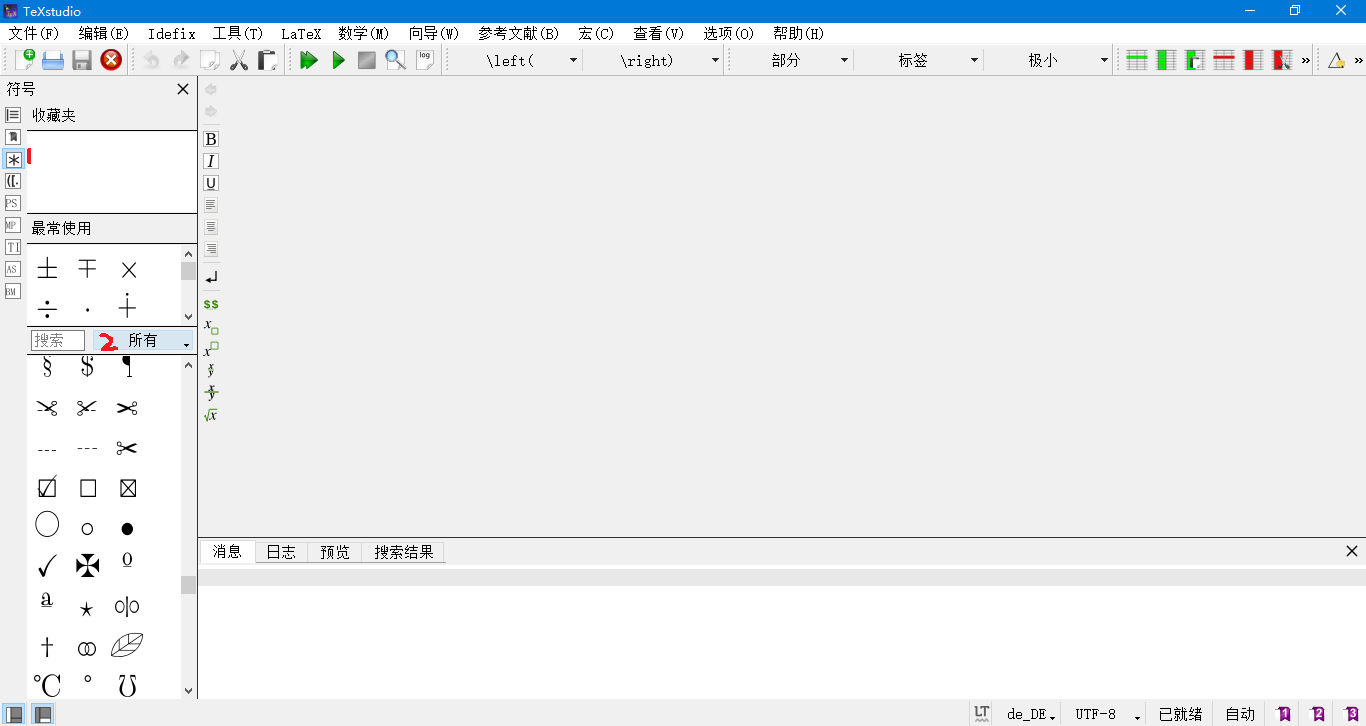
\includegraphics[width=0.9\textwidth]{include/images/5.png}
  \item 也可以手动输入,识别率不是特别高,可能需要多输入几次才会出来。设置如下:向导$\rightarrow$数学助手,手写输入完
  之后插入即可。

  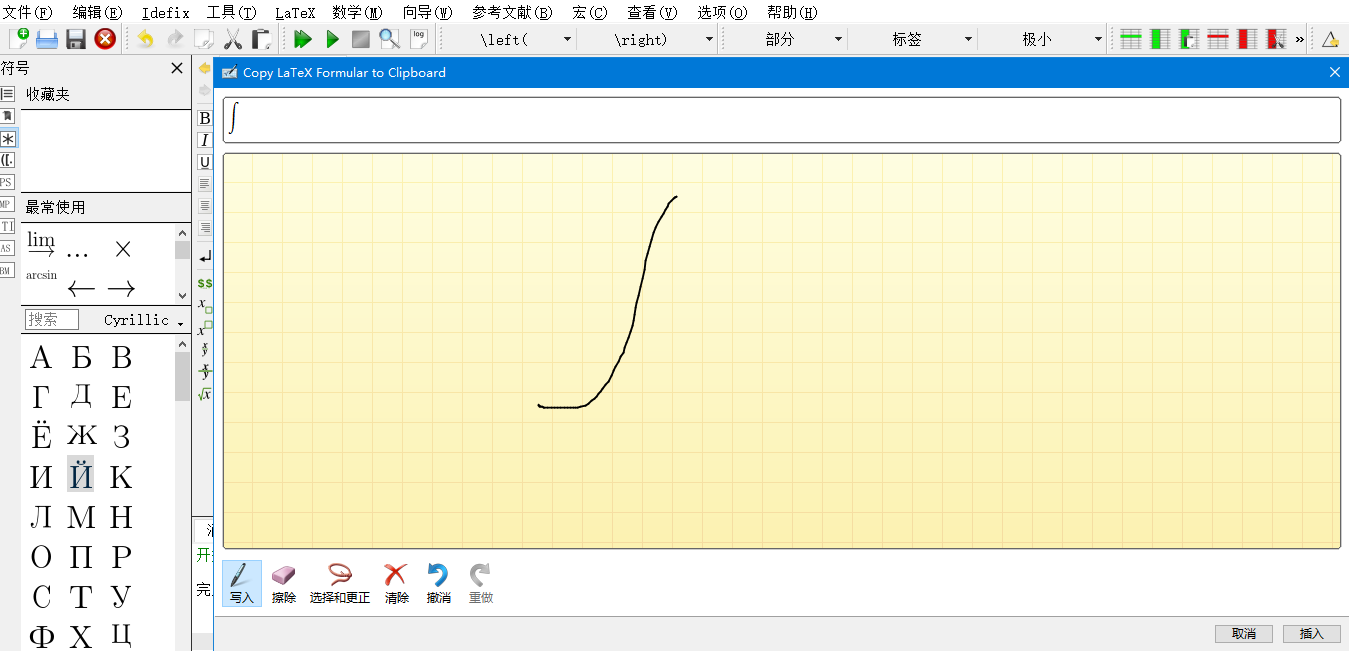
\includegraphics[width=0.9\textwidth]{include/images/image.png}
\end{itemize}


\faq{如何找到 FAQs}{}


\faq{如何控制章节编号的深度}{how-to-control-section-depth}

\LaTeX{} 标准文档类对章节划分了层级:
\begin{itemize}
  \item 在 article 文档类里 part 为0,section 为1,依此类推;
  \item 在 report/book 文档类里 part 为 $-1$,chapter 为0,section 为1,等等。
\end{itemize}

secnumdepth 计数器控制章节编号的深度,如果章节的层级大于secnumdepth,那么章节的标题、在目录和页眉页脚的标题都不编号
(照常生成目录和页眉页脚),章节计数器也不计数。可以用 |setcounter| 命令设置 secnumdepth 为较大的数使得层级比较深的
章节也编号,如设置为4令 |paragraph| 也编号;或者设置一个较小的数以取消编号,如设置为-1 令 |chapter| 不编号。
后者是生成不编号的章节的一个妙招,免去了手动使用 |addcontentsline| 和 |markboth| 的麻烦。
secnumdepth 计数器在 article 文档类里默认为3(subsubsection一级);在 report 和 book 文档类里默认为
2(subsection 一级)。

下面给出一个具体的例子:

\begin{verbatim}
  \documentclass{book}
  \setcounter{secnumdepth}{4}
  \begin{document}
    \part{part}
    \chapter{chapter}
    \section{section}
      \subsection{subsection}
      \subsubsection{subsubsection}
        \paragraph{paragraph}
  \end{document}
\end{verbatim}

控制目录页排版显示深度可以使用 |\setcounter{tocdepth}{2}|,此命令表示显示到三级标题。关于此问题的具体介绍可以参考
\href{https://blog.csdn.net/RobertChenGuangzhi/article/details/50480856}{该网页}。


\faq{如何下载 arXiv 上面的 \TeX{} 源文件}{how-to-download-arxiv-tex}
先访问 arXiv 上面的文章,在右边找到 Downloads $\rightarrow$ Other formats,点击进入下载页,点击 Download source。
将文件下载到本地后,重命名文件,文件后缀名是 .tar.gz。接下来解压缩 .tar.gz 文件,即可获得 \TeX{} 源文件。


\faq{Windows 系统下用 TeXstudio 打开中文编写的源文件遇到乱码怎么办}{windows-texstudio-chinese-GBK}

最简单的方法是借助 Notepad++ 等编辑器将文件转码为 UTF-8。如果没有 noteapd++,也可以直接使用 TeXstudio。
这里我们默认文件的编码是 GB2312。首先打开文件,在 TeXstudio 右下角找到 encoding 位置的内容,
有时系统显示为 ISO-8859-1。点击那里,进入 More encodings,在列表中点击 GB2312,然后点击按钮 view with。
正常来讲,乱码应该都会消失。 接下来,继续进入 More encodings,在列表中点击 UTF-8,然后点击按钮 change to。
经过这些操作,源文件就重新变成了 UTF-8 编码。


\faq{如何在listing抄录环境中显示公式}{how-to-listing-show-equations}

有时对抄录环境中的代码进行说明时,要用显示公式,这时只要进选项texcl设为true即可。

\begin{verbatim}
  \begin{lstlisting}[
    numbers=left,
    upquote=true,
    basicstyle=\ttfamily,
    texcl=true,
    language=Python
    ]
    #Generates Graphs $G^{(12)} ---  G^{(17)}$
    sGL6=['E@QW', 'EHQW', 'E@`w', 'E@]o', 'E@Rw', 'EAMw']
    GL=[Graph(s) for s in sGL6]
    \end{lstlisting}
\end{verbatim}
%  
%  % \begin{figure}
%  % \centering
%  % \includegraphics{https://images-cdn.shimo.im/LttXT6sECbcak9Qi/image.png!thumbnail}
%  % \caption{图片}
%  % \end{figure}
%  

或者设置mathescape~选项为true。

\begin{verbatim}
  \begin{lstlisting}[mathescape=true]
    if foo
    list= { $S_1,S_2,S_3$ }
  \end{lstlisting}
\end{verbatim}


\faq{能不能介绍一下排版试卷的方法与技巧,比如选择题,密封线设置等。}{how-to-latex-papers}


\faq{一个文档,如何在不同部分使用不同的页眉页脚}{how-to-set-different-geometry}

参考 geometry 宏包的自定义命令。比较常用的有如下四个命令
\begin{verbatim}
  \newgeometry{<options>}
  \restoregeometry
  \savegeometry{<name>}
  \loadgeometry{<name>}
\end{verbatim}
具体可参见该宏包的说明文档。


\faq{如何给中文文本加注音符号?}{how-to-pinyin}

xpinyin 宏包。


\faq{在book类文档中边注用什么宏包?边注的宽度能调整吗?}{book-geometry}


\faq{如何使用ctex相关类或者宏包制定章节样式,目录样式?}{ctex-tableofcontents}


\faq{如何给章节标题,目录列表加盒子边框?}{}


\faq{如何使用带圈数字?}{how-to-use-circle-number}

\begin{verbatim}
  \begin{enumerate}
    \def\labelenumi{\arabic{enumi}.}
    \setcounter{enumi}{7}
\end{verbatim}


\faq{如何改变列表标签样式,行距,缩进等各种相关间距?}{how-to-change-list-style}

enumitem 宏包


\faq{换行与换段的区别,有几种方式?}{change-line-paragraph}

换行是 |\\| 换段是 |\par|,或者空一行。
换行与分段最大的区别在于语义上是否形成一段完整的阐述、叙述,多读两遍你写的文字,如果你觉得问题没有叙述完,那么应该用换行,
反之则应该用分段。


\faq{在使用较早版本的CTeX里面附带的WinEdit出现打不开UTF-8编码文档的情况,如何处理?}{early-version-ctex-winedit-utf8}

使用记事本之类文本编辑器打开,转换编码方式另存一份即可。有时候需要注意BOM问题,一般没啥问题。


\faq{如何改变计数器样式为中文数字、罗马数字、阿拉伯数字或拉丁字母?}{how-to-change-listing-number}

可以通过重定义命令的方式修改默认的计数器样式,例如
\begin{verbatim}
  \renewcommand{\thechapter}{\Roman{chapter}}
\end{verbatim}
会将章序号计数器改为大写罗马数字计数形式。更多对应关系如下所示:

\begin{table}[h]
  \centering
  \begin{tabular}{cc}
    |\arabic| & 阿拉伯数字 \\
    |\alph| & 小写英文字母,数值应小于27 \\
    |\Alph| & 大写英文字母,数值应小于27 \\
    |\chinese| & 中文小写数字,需要调用\CTeX{}宏包 \\
    |\roman| & 小写罗马数字 \\
    |\Roman| & 大写罗马数字 \\
    |\fnsymbol| & 脚注标识符,数值应小于10
  \end{tabular}
\end{table}

详情可以参阅刘海洋、胡伟等编写的相应书籍,也可以查阅Wiki百科。


\faq{列表环境 (enumerate/itemize/description)的条目间距太大了,怎么改小一些?}{how-to-change-listing-linespace}

可以使用 paralist 宏包,它提供了一系列压缩了行间距的列表。对应的环境名称分别是 compactenum/compactitem/compactdesc,
也可以使用 enumitem 宏包修改三个列表环境的格式。


\faq{列表的条目项内容很短,可以让他们在一行内排版么?}{listing-short-oneline}

可以使用 paralist 宏包,这个宏包提供了 inparenum/inparitem/inpardesc 环境,可以在行内输出列表内容;
也可以带上 inline 选项使用 enumitem 宏包,可以使用带*形式的三个列表环境,即在行内输出列表内容。


\faq{enumerate宏包修改列表标签格式很方便,但是这个宏包和enumitem宏包冲突,有什么解决办法么?}{enumerate-fight-enumitem}

如果只是需要使用这种短标签表示方法,利用enumitem宏包同样能够做到,只需要带上shortlabels选项加载enumitem宏包即可。
同时,enumitem宏包提供了自定义短标签名称和格式的宏命令,你也可以自己定义一些有趣的标签形式。


\faq{如何使用带圈数字作为 enumerate 列表的标签?}{circle-number-enumerate}

\LaTeX{} 自带一个带圈字符的命令 |\textcircled|,不过,这个命令的排版效果非常差,几乎很少有人会直接使用。
带圈数字可以通过unicode字符实现,也可通过pifont宏包中|ding|命令实现(但是只能用到10以内的数字),
甚至可以通过tikz 自己绘制一个。使用带圈数字做enumerate的标签,可以通过 enumitem 宏包设置。
这里给出一个使用 unicode 字符实现带圈数字的方法,并将其应用于enumerate 的标签。

\begin{verbatim}
  \documentclass{article}
    \usepackage{xeCJK,xunicode,calc}
    \usepackage[shortlabels]{enumitem}
    \newcommand{\Cnum}[1]{%
    \ifnum #1<21
      \edef\a{\the\numexpr #1+9311}
    \else
      \ifnum #1<36
        \edef\a{\the\numexpr #1+12860}
      \else
        \ifnum #1<51
         \edef\a{\the\numexpr #1+12941}
        \else
          \PackageError{your package}{Number too large}{}
        \fi
      \fi
    \fi
    {\CJKfontspec{Noto Serif CJK SC}\fontspec{Noto Serif CJK SC}\symbol\a}}
    \SetEnumerateShortLabel{o}{\protect\Cnum{\arabic*}}
    \begin{document}
    \Cnum{12} \Cnum{32} \Cnum{46} 
    
    \begin{enumerate}[o]
      \item The first item.
      \item The second item.
      \item The Third One.
    \end{enumerate}
    \end{document}
\end{verbatim}


\faq{如何给目录中的章节都带上引导点来连接页码?}{tableofcontents-dotdotdot}

其实级别较高的章节结构,如book/report中的chapter和arcticle中的section,是不需要这种引导点来连接页码的,有这种需求
的多是受Microsoft Word的影响。如果一定要这种引导点,可以在导言区增加这样一段代码。
\begin{verbatim}
  \makeatletter
  \def\@bfdottedtocline#1#2#3#4#5{%
  \ifnum #1>\c@tocdepth \else
  \vskip \z@ \@plus.2\p@
  {\leftskip #2\relax \rightskip \@tocrmarg \parfillskip -\rightskip
  \parindent #2\relax\@afterindenttrue
  \interlinepenalty\@M
  \leavevmode \bfseries
  \@tempdima #3\relax
  \advance\leftskip \@tempdima \null\nobreak\hskip -\leftskip
  {#4}\normalfont\nobreak
  \leaders\hbox{$\m@th
  \mkern \@dotsep mu\hbox{.}\mkern \@dotsep
  mu$}\hfill
  \nobreak
  \hb@xt@\@pnumwidth{\hfil\normalfont \normalcolor #5}%
  \par}%
  \fi}
  \renewcommand*\l@section{\@bfdottedtocline{0}{0em}{1.5em}}
  \makeatother
\end{verbatim}
当然,最后一句应根据实际的文档类型来重定义 |\l@chapter| 或 |\l@section|。


%\begin{faq}{如何临时切换页面大小?}
%
%  \begin{enumerate}
%    \def\labelenumi{\arabic{enumi}.}
%    \setcounter{enumi}{1}
%
%    \item
%    没有编号的章节标题如何添加到目录里?
%  \end{enumerate}
%
%  使用
%  \begin{verbatim}
%  \addcontentsline{toc}{⟨level⟩}{⟨title⟩}
%  \end{verbatim}
%
%  ;举个例子:
%  \begin{verbatim}
%  \section*{译者序}\addcontentsline{toc}{section}{译者序}
%  \end{verbatim}
%
%  这样在目录中译者序是没有编号的,对应等级是section,标题是译者序
%  参考:《lshort》目录章节 3. 怎样定义 第几页/共几页 的页码样式?
%
%  可以调用末页标签宏包lastpage,并将页码设置如下:
%
%  \begin{verbatim}
%  第 \thepage 页 / 共 \pageref{LastPage} 页
%  \end{verbatim}
%
%  如果不想调用这个宏包,还可以自己DIY,虽然ugly,但是可以达到目的 ):
%  在文档末尾设置一个标签,例如在 \verb|\end{doucument}| 前加一句
%  \verb|\label{AllPage}|,然后将页码设置为:
%
%  \begin{verbatim}
%  第 \thepage 页 / 共 \pageref{AllPage} 页
%  \end{verbatim}
%
%  \begin{enumerate}
%    \def\labelenumi{\arabic{enumi}.}
%    \setcounter{enumi}{3}
%
%    \item
%    超链接如何断行?
%  \end{enumerate}
%
%  先写
%
%  \begin{verbatim}
%  \PassOptionsToPackage{hyphens}{url}
%  \end{verbatim}
%
%  再写
%
%  \begin{verbatim}
%  \usepackage{hyperref}
%  \end{verbatim}
%\end{faq}
%
%
%\begin{faq}{在使用较早版本的CTeX里面附带的winedt出现打不开utf8编码文档的情况,如何处理?}
%
%  使用记事本之类文本编辑器打开,转换编码方式另存一份即可。有时候需要注意BOM问题,一般没啥问题。
%  2. 如何在axmath转换代码到texstudio?
%
%  点击下图中第10个按钮,即可将数学公式转换为LaTeX代码,复制即可。
%  % \includegraphics{https://images-cdn.shimo.im/oMh77ZPr7iIsh2tB/image.png!thumbnail}
%  3.
%  双栏文档中,如何可以让左边先写完,然后再切换到右边,而不是左右一样长?
%
%  如果是采用文档类 twocolumn
%  选项实现的双栏模式,正文的排版就是先将左边排完,再从右边开始排。而采用
%  multicol 宏包的 muticols 环境则是左右两边底部对齐的。 4.
%  如何输入中文破折号?
%
%  输入法输入咯,英文的破折号 --- 用于中文不合适。 5.
%  \cs{input} 和 \cs{include} 有何区别? * \cs{include}
%  在读入文件之前会另起一页。\cs{input}
%  命令纯粹是把文件里的内容插入 * \cs{include}不可用于导言区
%\end{faq}
%
%
%\begin{faq}{subfiles有什么用?}
%
%  \begin{enumerate}
%    \def\labelenumi{\arabic{enumi}.}
%    \setcounter{enumi}{1}
%
%    \item
%    ~如何使用latexmk编译文档?
%    \item
%    定理环境要怎么使用?
%    \item
%    算法环境如何使用?
%    \item
%    在lstlisting环境中如何输出破折号?
%    \item
%    minted里面tab键为什么会输出成\^{}\^{}T,如何解决?
%    \item
%    一段代码粘贴到texstudio里面就没有了缩进,如何解决?
%    \item
%    在LaTeX或Tikz中,能否输入随机且字数随机可控的文字?
%    \item
%    如何输入罗马数字等?
%    \item
%    如何在等号中插入问号?
%  \end{enumerate}
%
%  \begin{verbatim}
%  \stackrel{?}{=}.
%  \end{verbatim}
%\end{faq}
%
%
%\begin{faq}{如何在插入的图片上标记引注?}
%
%  \begin{enumerate}
%    \def\labelenumi{\arabic{enumi}.}
%    \setcounter{enumi}{1}
%
%    \item
%    如何让一个很长很长的字符串(中间不带空格)自动换行?
%    \item
%    \cs{bf} \cs{sf} \cs{it} \cs{sl} 这些命令都很短小,为什么不建议继续使用了?
%    \item
%    如何自动化打包 LaTeX
%    文档发送给别人以确保宏包、字体是完整的,便于他人顺利编译、减少麻烦。
%    \item
%    如何编译网站上下载的他人的模板,一般是不知道对应的编译器应该选择什么,还有编译顺序是什么,希望在提供模板的同时说明应该如何编译。
%    \item
%    我以book文档类为基础新写一个文档类,book文档类的选项会自动适用于我新建的文档类么?
%    \item
%    \cs{def} 和 \cs{newcommand}
%    有什么区别,我创建新命令的时候究竟应该用哪个?
%    \item
%    怎样创建一个带*的命令?
%    \item
%    ~类似 \verb|\macro[<option1>][<option2>]{<arg>}|
%    这样的宏命令,当我只使用一个可选参数时,LaTeX
%    把它看做哪个参数?LaTeX会自动判断么?
%    \item
%    \cs{newcommand}
%    创建的命令,仅有第一个命令可以成为可选参数,如果我想创建具有两个可选参数的命令,应该如何去写?
%    \item
%    有些命令的参数是使用( ) 扩起来的,这类命令是如何定义的?
%    \item
%    我想新建一个带有可选参数的命令,可选参数的缺省值与必选参数值一样,这样的命令如何创建?
%    \item
%    想用minted包写文档,怕别人用不来不会设置-shell --escepe咋办
%    \item
%    .latex如何给整个页面加边框?
%  \end{enumerate}
%\end{faq}

% % Copyright (C) 2018 by latexstudio <http://www.latexstudio.net>
%
% This program is free software: you can redistribute it and/or modify
% it under the terms of the GNU General Public License as published by
% the Free Software Foundation, either version 3 of the License, or
% (at your option) any later version.
%
% This program is distributed in the hope that it will be useful,
% but WITHOUT ANY WARRANTY; without even the implied warranty of
% MERCHANTABILITY or FITNESS FOR A PARTICULAR PURPOSE.  See the
% GNU General Public License for more details.
%
% You should have received a copy of the GNU General Public License
% along with this program.  If not, see <http://www.gnu.org/licenses/>.
%

\section{介绍公式的常见问题。}
%\end{faq}
%
%
%\begin{faq}{\cs{ldots} 与...有什么区别?}
%
%重定义的难度不同、造成的间距也不同。推荐使用 {[}\ldots{}{]}。 见
%\url{https://www.zhihu.com/question/27589739/answer/37255728}
%\end{faq}
%
%
%\begin{faq}{如何让长公式自动断行?}
%
%长公式自动断行要看情况,如果是在行内模式,合理使用空格,一般可以在二元运算符处断行,如果是行间模式,推荐使用align类环境,在需要断行处添加
%\textbackslash{} 手动断行。
%\end{faq}
%
%
%\begin{faq}{公式希腊字符如何加粗?}
%
%希腊字母没有粗体,可以选择合适的数学字体。 可以使用 bm
%宏包将希腊字母加粗。
%\end{faq}
%
%
%\begin{faq}{极限符号下面有两个趋近该怎么写}
%
%直接给出例子:
%
%\begin{verbatim}
%\documentclass{article}
%\begin{document}
%\[ \lim_{n\to\infty\atop m\to\infty} \]
%\end{document}
%\end{verbatim}
%
%或者使用 \cs{substack},代码如下:
%
%\begin{verbatim}
%\documentclass{article}
%\usepackage{amsmath}
%\begin{document}
%\[ \lim_{\substack{n\to\infty\\ m\to\infty}} \]
%\end{document}
%\end{verbatim}
%
%效果如下:
%% \includegraphics{https://images-cdn.shimo.im/FCY4A1SeBIcwBCGT/双重极限.PNG!thumbnail}
%\end{faq}
%
%
%\begin{faq}{怎样在 LaTeX
%  中输入引号}
%
%左引号用 `(键盘1旁边那个键),右引号用 `。双引号也一样,``''。
%中文条件下可以直接用中文引号(这个与编码方式和中文支持方式有关的),会有自动配对(这个和编辑器以及输入法有关的),但是如果需要用到不配对引号的情况,需要使用通用方法。
%\end{faq}
%
%
%\begin{faq}{align环境默认是居中对齐吗?我在使用时,发现公式开始是居中的,后来却一直靠右断对齐,这是什么原因?}
%
%\sout{align 默认靠右对齐,所以通常加 \&
%  符号,让代码左对齐。验证一下以下代码:}
%
%\begin{verbatim}
%\begin{align}
%& \nabla \times H = J,\\
%& \nabla \times E = - \partial _t B,\\
%& \nabla \cdot B = 0.
%\end{align}
%\end{verbatim}
%
%再试试把 \& 去掉什么样。
%align采用的是奇偶对齐的方式,第一列右对齐,第二列左对齐,就这样右左右左依此类推,两列之间用\&分隔。
%\end{faq}
%
%
%\begin{faq}{中英文标点使用规则不是很明白,尤其在公式环境里,字体和间距差别都比较大。怎样才能让正文和公式的标点统一(形状和间隔)?}
%
%详见:
%\url{https://link.zhihu.com/?target=http\%3A//www.moe.gov.cn/ewebeditor/uploadfile/2015/01/13/20150113092346124.pdf}
%在导言区加类似命令可实现全文替换:
%
%\begin{verbatim}
%\catcode`\。=\active\newcommand{。}{. }
%\end{verbatim}
%
%或者使用 xeCJK 宏包的字符映射功能,调用 fullwidth-stop
%这一映射文件,将中文空心句号映射为实心句点:
%
%\begin{verbatim}
%\documentclass{article}
%\usepackage{xeCJK}
%\setCJKmainfont[Mapping= fullwidth-stop]{STSong}
%\begin{document}
%句号。
%\end{document}
%\end{verbatim}
%\end{faq}
%
%
%\begin{faq}{公式如何居左对齐,居右对齐?}
%
%公式居左对齐在基础文档类中由 fleqn
%选项控制,选择该选项后,正文公式均居左对齐,至于居右对齐,嗯,我没见过这么奇怪的格式。
%\end{faq}
%
%
%\begin{faq}{公式之后解释公式符号的文字,通常是 ``符号 ------ 解释''
%  这样的格式,我希望这段文字的格式是按破折号对齐,并且解释文字折行后悬挂缩进,怎样实现这样的格式?}
%
%方法很多,可以列表,可以align等环境。 这里给出一个使用自定义列表的例子:
%
%\begin{verbatim}
%\usepackage{ifthen}
%\newcounter{qlst}
%\newenvironment{EqDesc}[2][式中]{%
%\begin{list}{}
%{%
%\usecounter{qlst}
%\settowidth{\labelwidth}{#1,#2\ --- \ }
%\setlength{\labelsep}{0pt}
%\setlength{\leftmargin}{\labelwidth}
%\setlength{\rightmargin}{0em}
%\setlength{\parsep}{0ex}
%\setlength{\itemsep}{0ex}
%\setlength{\itemindent}{0em}
%\setlength{\listparindent}{0em}
%\renewcommand{\makelabel}[1]{\stepcounter{qlst}\ifthenelse{\value{qlst}>1}{\hfill ##1\ --- \ 
%}{#1,\hfill ##1\ --- \ }}
%}}%
%{\end{list}}%
%\end{verbatim}
%
%EqDesc
%环境有两个参数,第一个为可选参数,是解释公式符号前的引导词,默认是``式中'',第二个参数是样本符号,可以选择一个列表中宽度最大的符号。条目
% \cs{item} 有一个可选参数(实际使用是必选参数),内容是要说明的符号。使用如下:
%
%\begin{verbatim}
%\[ a^2+b^2=c^2 \]
%\begin{EqDesc}[其中]{$a$}
%\item[$a$] 三角形的一条直角边;
%\item[$b$] 三角形的另一条直角边;
%\item[$c$] 三角形的斜边。
%\end{EqDesc}
%\end{verbatim}
%\end{faq}
%
%
%\begin{faq}{行内公式的情况下如何让sum
%  prod这些运算符的上下标在头上和脚下?}
%
%这样处理行内公式的上下标会导致段落行距不整齐,不符合 LaTeX
%的审美。如果彻底放弃审美,可以使用 \cs{limits} 命令,如:
%
%\begin{verbatim}
%$\sum\limits_{i=1}^n \quad
%\prod\limits_\epsilon$
%\end{verbatim}
%\end{faq}
%
%
%\begin{faq}{如何将积分的上限标放在积分号的上下两侧?}
%
%积分号的上下限放置在积分号的右侧是英美国家和 LaTeX
%的排版习惯,通常无需处理。如果你很确定需要按照 ISO 80000-2:2009 或者 GB
%3102.11-93 的规定排版积分号,可以:
%
%\begin{enumerate}
%  \def\labelenumi{\arabic{enumi}.}
%  
%  \item
%  在调用 amsmath 宏包时添加 intlimits 选项;
%  \item
%  \texttt{\textbackslash{}def\textbackslash{}int\{\textbackslash{}intop\}}
%  \item
%  如果使用 unicode-math 宏包,
%\end{enumerate}
%
%\begin{verbatim}
%\removenolimits{%
%\int\iint\iiint\iiiint\oint\oiint\oiiint
%\intclockwise\varointclockwise\ointctrclockwise\sumint
%\intbar\intBar\fint\cirfnint\awint\rppolint
%\scpolint\npolint\pointint\sqint\intlarhk\intx
%\intcap\intcup\upint\lowint
%}
%\end{verbatim}
%\end{faq}
%
%
%\begin{faq}{如何自定义数学运算符,然后让下标放在脚下?}
%
%借助 amsmath 包的
%\cs{DeclareMathOperator*} 命令即可(需要注意加不加*是有区别的)。例如
%
%\begin{verbatim}
%\DeclareMathOperator*{\esssup}{ess\,sup}
%\end{verbatim}
%\end{faq}
%
%
%\begin{faq}{在数学公式中,编辑等式时,每一行需要等号和等号对其,这时使用了\textbackslash{}begin\{displaymath\}
%  \textbackslash{}begin\{split\}环境,但是呢,这些整体都是居中的,我想让式子靠左,怎么实现呢?}
%\end{faq}
%
%
%\begin{faq}{行列式变换过程中,我们一般是在中间的箭头上表示出变换的方式,如何才能在长箭头上打出多行内容?}
%\end{faq}
%
%
%\begin{faq}{如何输出反斜杠?}
%
%\begin{verbatim}
%\textbackslash \verb|\|
%\end{verbatim}
%\end{faq}
%
%
%\begin{faq}{对equation环境下的公式、图片编号按章节、小节进行重新定义}
%\end{faq}
%
%
%

% % Copyright (C) 2018 by latexstudio <http://www.latexstudio.net>
%
% This program is free software: you can redistribute it and/or modify
% it under the terms of the GNU General Public License as published by
% the Free Software Foundation, either version 3 of the License, or
% (at your option) any later version.
%
% This program is distributed in the hope that it will be useful,
% but WITHOUT ANY WARRANTY; without even the implied warranty of
% MERCHANTABILITY or FITNESS FOR A PARTICULAR PURPOSE.  See the
% GNU General Public License for more details.
%
% You should have received a copy of the GNU General Public License
% along with this program.  If not, see <http://www.gnu.org/licenses/>.
%

\section{参考文献篇}


\faq{参考文献中的特殊字符或字母}{}


\faq{BibTeX 不理解的作者列表}{}

BibTeX 只支持三种姓名格式: * First von Last * von Last, First * von
Last, Jr, First

多个姓名之间必须使用``and''连接,如

\begin{verbatim}
author = {Knuth, Donald E. and Lamport, Leslie},
\end{verbatim}


\faq{BibTeX 排序和名字前缀}{}


\faq{BibTeX 中的大写字母}{}

英文标题中常使用的大小写方式有:

\begin{enumerate}
\def\labelenumi{\arabic{enumi}.}

\item
  Title case:
  句首字母大写,并且除冠词、连词和短介词以外的词首字母大写,这里说的``短''介词一般指不超过
  4 个字母的介词。比如``The Quick Brown Fox Jumps over the Lazy Dog'';
\item
  Sentence case:
  句首字母和一些专有名词的首字母大写,同普通的英文句子大小写方式一样,如``The
  quick brown fox jumps over the lazy dog''。
\end{enumerate}

BibTeX 根据 bst 样式文件可以将题名保留原大小写,或转为 sentence
case。所以用户在 bib 数据库中著录标题的正确方式是,统一使用 title
case,并将需要专有名词用大括号括起来。

\begin{verbatim}
title = {Finite Element Methods for {Maxwell's} Equations},
\end{verbatim}

注意尽量避免将一个词中个别字母用大括号括起来,如``\{M\}axwell's'',这可能会导致字母的间距有问题,建议将整个词括起来,如``\{Maxwell's\}''。


\faq{如何选择参考文献的风格}{}

参考文献的风格一般是期刊或会议模板指定 bst
的,作者应仔细阅读投稿要求和模板使用说明,根据规定使用合适的
bst。通常有以下方式:

\begin{enumerate}
\def\labelenumi{\arabic{enumi}.}

\item
  在文档中声明 |\bibliographystyle{ieeetran}|
\item
  在模板的文档类选项中使用合适的参数,如 |\documentclass[authoryear]{ustcthesis}|。
\end{enumerate}


\faq{BibTeX 参考文献数据库}{}

BibTeX 的 bib 文件是一个记录已阅文献的数据库,但是通常不建议手动编译 bib
文件,建议:

\begin{enumerate}
\def\labelenumi{\arabic{enumi}.}

\item
  使用 JabRef 或 Zotero 等文献管理工具导出 bib 文件创
\item
  使用 \href{https://scholar.google.com/}{Google Scholar} 或
  \href{https://cn.bing.com/academic}{Bing 学术}导出 bib 条目建
\end{enumerate}


\faq{创建参考文献风格}{}

BibTeX 的风格文件 bst
是使用一种后缀语言写的代码,如果对编程能力比较自信的话,可以阅读 BibTeX
的文档 btxdoc 和 btxhak,btxbst.doc 文件提供了标准 bst
风格的代码注释,另外还可以阅读 ttb 和 The LaTeX Companion 等资料。

如果不习惯 bst 的编程语言,可以使用 custom-bib 工具,在命令行下运行latex
makebst,回答一系列问题生成自己的bst。

另外还可以考虑使用 biblatex,它提供更方便的接口用于自定义参考文献格式。


\faq{参考文献中的数字格式}{}

参考文献表中的数字格式是由 @biblabel
控制的,可以通过重定义该命令来修改格式。比如将数字修改为左对齐:

\begin{verbatim}
\makeatletter
\renewcommand\@biblabel[1]{[#1]\hfill}
\makeatother
\end{verbatim}


\faq{BibTeX文献条目列表}{}

科技论文通常要求参考文献表中的文献必须在正文中引用,但是在某些特殊情况下仅需要列出
bib 数据库中的文献,可以使用 |\nocite{*}|
命令列出调用的bib中所有条目,或者使用类似 |\nocite{ref1,ref2,ref3}| 命令列出需要显示的条目。


\faq{制作参考文献的HTML}{}


\faq{BibTeX中的多字母缩写}{}


\faq{多个参考文献表}{}

natbib宏包与Donald Arseneau和Niel
Kempson编写的chapterbib宏包兼容,该宏包允许在一个文档内有多个独立的参考文献列表。通常用法是一本书的各章有独立的参考文献列表,尤其是在各章由不同作者独立编写时。


\faq{同一位置多文献引用}{}

只需要将多篇文献的bibkey用英文半角逗号分隔写在一个cite指令的选项里即可。如:

\begin{verbatim}
\cite{knuth84,lamport86}
\end{verbatim}


\faq{非英文参考文献条目}{}

什么叫非英文参考文献条目?是指bibkey么?一般不建议用中文,处理好编码格式,无殊。
中文的参考文献条目,与英文条目并没有什么差别,只是注意编码。目前处理中文推荐用xelatex
编译 utf8 编码的文件。因此中文的 bib 条目也应该用 utf8 编码。


\faq{BibTeX 文献手写很困难,有没有什么工具能够生成?}{}

多数时候,我们无需自己手写 BibTeX 文献条目。从
\url{https://scholar.google.com/}、\url{https://academic.microsoft.com/}、
\url{https://cn.bing.com/academic?mkt=zh-CN}
或者期刊、数据库的网站上都能够导出 BibTeX 文献条目。 老牌的文献管理软件
EndNote 也支持生成 BibTeX 格式的数据库,详情见
官网\url{https://endnote.com/}。 开源软件 JabRef 甚至支持 BibTeX
文献条目的导入、导出和管理,详情见 官网\url{http://www.jabref.org/}。
Zetero 使用起来也非常方便,详情见官网 \url{https://www.zotero.org/}。
谷歌学术、知网、百度学术、万方数据库等在线数据库也是可以支持导出 .bib
文件的,至于哪家的数据条目更全,就得你自己去甄别了。


\faq{如何使用 BibTeX 排版参考文献}{}

\begin{itemize}

\item
  准备一份 BibTeX 数据库,假设数据库文件名为 books.bib,和 LaTeX
  源代码一般位于同一个目录下。
\item
  在源代码中添加必要的命令,如

  \bibliographystyle{abbrv}

  ,

  \bibliography{books}

  。假设源代码名为 demo.tex。其中,

  \cs{bibliographystyle}

  设定参考文献的格式。\textbackslash{}bibliography
  告诉系统使用哪个数据库和参考文献列在哪个位置。
\item
  写好了以上两个文件之后,我们就可以开始编译了。例如在命令行中执行以下命令
\end{itemize}

\begin{verbatim}
xelatex demo
bibtex demo
xelatex demo
xelatex demo
\end{verbatim}

或者选择一个可以自动检测是否有参考文献的编辑器,如果有,它会自动执行以上四个命令,但是有时候会遇到检测不到的情况,这时你只需要清理一下辅助文件即可。


\faq{如何将参考文献条目录入到正文中}{}

理工科类论文很少用。


\faq{bib文件的重建}{}

用文本编辑器如Notepad++, Sublime
Text或WinEdt或专门文献管理软件JabRef,BibDesk等创建文件,改名为 ref.bib
文件,往里头添加参考文献目录。参考如下:
% \includegraphics{https://images-cdn.shimo.im/VKQ8uAycksg1zPlo/image.png!thumbnail}
在.bib文件中,可以采用 TeXStudio 提供的参考文献格式,在自行修改内容
% \includegraphics{https://images-cdn.shimo.im/0OgCsRQoufMTDJ75/1.png!thumbnail}
上面的类型有两种选择 BibTeX 和 BibLaTeX ,后者的选择更为广泛。
参考文献一般不自己书写,而是有可以直接导入。 一般直接 Google
学术搜索出来的文献或者引用知网,如下:
% \includegraphics{https://images-cdn.shimo.im/L1fAEZmW9tYDVTYT/VRI1FEC62J_C6_QSK_P0_0.png!thumbnail}
点击上图红圈的引号-\textgreater{}
% \includegraphics{https://images-cdn.shimo.im/N8tFzuXsCM8rOPjF/image.png!thumbnail}
在点击最左侧的 BibTeX -\textgreater{}
% \includegraphics{https://images-cdn.shimo.im/81Z6BGei8ycQf1uK/image.png!thumbnail}
将其复制黏贴到你的 ref.bib 文件中即可。
在知网上的文献查询需要下载安装如下软件:
% \includegraphics{https://images-cdn.shimo.im/ZsikCVGdjGIKBqSN/image.png!thumbnail}
两个都装好了之后,该软件需要自行注册登陆使用。
然后打开知网,会看到如下:
% \includegraphics{https://images-cdn.shimo.im/DVEoaSyHJKwmbSjH/2.png!thumbnail}
右上角红圈圈到的就是为浏览器安装的 Zotero Connector插件,在此需要打开
Zotero
软件,点击之后显示下图,选择需要的文献。
% \includegraphics{https://images-cdn.shimo.im/w4eu1WOehS05gJ0g/image.png!thumbnail}
然后 Zotero 软件如下显示
% \includegraphics{https://images-cdn.shimo.im/VFUjYs5MvKQz522e/image.png!thumbnail}
然后文件-\textgreater{}导出文献库-\textgreater{}导出格式 BibTeX
确定保存生成的bib文件,可以将这个 bib 文件中的参考文献全部复制黏贴到你的
ref.bib
文件中,也可以单独作为一个新的bib文件,在正文区则需要添加多个bib文件就可以,用命令
\begin{verbatim}
\bibliography{test,ref}
\end{verbatim}

,多个bib文件用逗号分隔即可。同时为引用的参考文献需要命令 \nocite{*}
来将未引用的文件全部排版出来。 注:百度学术、万方数据库等也支持导出 .bib
文件。


\faq{如何减少参考文献条目行间距}{}

文献条目间距为 \cs{itemsep},默认值4.5pt plus 2pt minus
1pt,可通过指令 |\addtolength{\itemsep}{距离}| 调整。


\faq{按照章节分开参考文献条目}{}

可看看chapterbib宏包。 \#\# 引文的排序及压缩

这个取决于使用的宏包,常用的natbib宏包可以使用sort或者sort\&compress选项激活相应的排序或排序并压缩功能。
\#\# 引文列表排序

这个取决于bst,一般模板都有指定的bst。 \#\# BibTeX中过长的字符串 \#\#
按照``unsrt''规则的目录重排序 \#\# BibTeX参考文献中的URL

调用url或者xurl宏包即可正常使用url,也可以看看href宏包。 \#\# 基于Plain
TeX的BibTeX的使用 \#\# 常用的biblatex参考文献样式

biblatex除了可以应用自带的标准样式外,还可以使用其他作者提供的第三方样式,这里介绍一些常用的样式:
* 国外常用 * APA * MLA * 国内 * GB7714-2015
样式名\textbar{}用法\textbar{}对应的bibtex样式\textbar{}作者介绍\textbar{}样式说明\textbar{}
:----:\textbar{}:----:\textbar{}:----:\textbar{}:----:\textbar{}:----:\textbar{}
trad-plain\textbar{}\texttt{\textbackslash{}usepackage{[}style=trad-plain{]}\{biblatex\}}\textbar{}plain\textbar{}MarcoDaniel
and
MoritzWemheuer,后者是biblatex维护者之一\textbar{}将引文按字母顺序排序,比较次序为作者姓氏、出版年份和题名,如果不能顺序,将以在正文中的引用顺序为准。\textbar{}
trad-unsrt\textbar{}\texttt{\textbackslash{}usepackage{[}style=trad-unsrt{]}\{biblatex\}}\textbar{}unsrt\textbar{}MarcoDaniel
and
MoritzWemheuer\textbar{}按照在正文中引用文献的先后顺序排列文献,其排版格式与trad-plain基本相同\textbar{}
trad-alpha\textbar{}\texttt{\textbackslash{}usepackage{[}style=trad-alpha{]}\{biblatex\}}\textbar{}alpha\textbar{}MarcoDaniel
and
MoritzWemheuer\textbar{}用文献的作者姓氏前三个字母加出版年份的后两位数作为文献序号,如果出现相同的序号,则会根据排序结果在序号后追加字母以示区别,排序方法和排版格式与trad-plain相同\textbar{}
trad-abbrv\textbar{}\texttt{\textbackslash{}usepackage{[}style=trad-abbrv{]}\{biblatex\}}\textbar{}abbrv\textbar{}MarcoDaniel
and MoritzWemheuer\textbar{}将文献中作者名和月份名的拼写改为缩写,
显得文献信息紧凑简洁, 其排序方法和排版格式与trad-plain相同\textbar{}
ieee\textbar{}\texttt{\textbackslash{}usepackage{[}style=ieee{]}\{biblatex\}}\textbar{}IEEEtran\textbar{}Joseph
Wright,biblatex
维护者之一\textbar{}国际电气电子工程师协会IEEE期刊文献格式\textbar{}
apa\textbar{}\texttt{\textbackslash{}usepackage{[}style=apa{]}\{biblatex\}}\textbar{}apalike\textbar{}Philip
Kime,biblatex 作者之一\textbar{}American Psychological Association
的文献格式\textbar{}
Chicago\textbar{}\texttt{\textbackslash{}usepackage\{biblatex-chicago\}}\textbar{}Chicago\textbar{}David
Fussner\textbar{}for the Chicago Manual of Style\textbar{}
iso-numeric\textbar{}\texttt{\textbackslash{}usepackage{[}style=iso-numeric{]}\{biblatex\}}\textbar{}
\textbar{}Michal Hoftich\textbar{}ISO690 international standard numeric
system\textbar{}
iso-iso-authoryear\textbar{}\texttt{\textbackslash{}usepackage{[}style=iso-iso-authoryear{]}\{biblatex\}}\textbar{}
\textbar{}Michal Hoftich\textbar{}ISO690 international standard
nameanddate system,so-called Harvard style\textbar{}
gb7714-2015\textbar{}\texttt{\textbackslash{}usepackage{[}style=gb7714-2015{]}\{biblatex\}}\textbar{}gbt7714-unsrt.bst
by zepinglee\textbar{}hushidong\textbar{}中文文献著录标准 GB/T 7714-2015
顺序编码制\textbar{}
gb7714-2015ay\textbar{}\texttt{\textbackslash{}usepackage{[}style=gb7714-2015ay{]}\{biblatex\}}\textbar{}gbt7714-plain.bst
by zepinglee\textbar{}hushidong\textbar{}中文文献著录标准 GB/T 7714-2015
著者年份制\textbar{}
caspervector\textbar{}\texttt{\textbackslash{}usepackage{[}style=caspervector{]}\{biblatex\}}\textbar{}
\textbar{}Casper vector\textbar{}一种中文文献格式\textbar{}
nature\textbar{}\texttt{\textbackslash{}usepackage{[}style=nature{]}\{biblatex\}}\textbar{}
\textbar{}Joseph Wright\textbar{}for Nature\textbar{}
science\textbar{}\texttt{\textbackslash{}usepackage{[}style=science{]}\{biblatex\}}\textbar{}
\textbar{}Joseph Wright\textbar{}for Science\textbar{}
chem-acs\textbar{}\texttt{\textbackslash{}usepackage{[}style=chem-acs{]}\{biblatex\}}\textbar{}
\textbar{}Joseph Wright\textbar{}covers most American Chemistry Society
journals\textbar{}
chem-angew\textbar{}\texttt{\textbackslash{}usepackage{[}style=chem-angew{]}\{biblatex\}}\textbar{}
\textbar{}Joseph Wright\textbar{}covers Angewandte Chemie Chemistry--A
European Journal.\textbar{}
chem-biochem\textbar{}\texttt{\textbackslash{}usepackage{[}style=chem-biochem{]}\{biblatex\}}\textbar{}
\textbar{}Joseph Wright\textbar{}covers Biochemistry and asmallnumber of
other American Chemistry Society journals\textbar{}
chem-rsc\textbar{}\texttt{\textbackslash{}usepackage{[}style=chem-rsc\ {]}\{biblatex\}}\textbar{}
\textbar{}Joseph Wright\textbar{}covers all Royal Society of Chemistry
journals\textbar{}
phys\textbar{}\texttt{\textbackslash{}usepackage{[}style=phys{]}\{biblatex\}}\textbar{}
\textbar{}Joseph Wright\textbar{}for AIP and APS\textbar{}
nejm\textbar{}\texttt{\textbackslash{}usepackage{[}style=nejm{]}\{biblatex\}}\textbar{}
\textbar{}MarcoDaniel\textbar{}for New England Journal of
Medicine\textbar{}
mla\textbar{}\texttt{\textbackslash{}usepackage{[}style=mla{]}\{biblatex\}}\textbar{}
\textbar{}James Clawson\textbar{}for Modern Language
Association\textbar{}
authortitle-dw\textbar{}\texttt{\textbackslash{}usepackage{[}style=authortitle-dw{]}\{biblatex\}}\textbar{}
\textbar{}Dominik Waßenhoven\textbar{}for Humanities\textbar{}
footnote-dw\textbar{}\texttt{\textbackslash{}usepackage{[}style=footnote-dw{]}\{biblatex\}}\textbar{}
\textbar{}Dominik Waßenhoven\textbar{}for Humanities\textbar{}


\faq{使用超链接,如何去除颜色边框?}{}

直接在引用 hyperref 宏包的时候使用以下命令之一

\begin{verbatim}
\usepackage[hidelinks]{hyperref}
\usepackage[colorlinks]{hyperref}
\end{verbatim}

第一种方法是隐藏链接,即隐藏颜色和边框。
第二种方法是用不同颜色来替换默认的边框强调超链接的方式,但是这种方法会使得链接具有不同的颜色。如果需要设置各种链接的颜色可以参考
hyprref
的说明文档,值得庆幸的是,该宏包已经有了一个\href{https://github.com/latexstudio/LaTeXPackages-CN/blob/master/hyperref/hyperref-zh-cn.pdf}{中文翻译版}。


\faq{参考文献列表行距如何设置?}{}

设置好文献条目间距 \cs{itemsep} 即可。


\faq{参考文献编号如何左对齐,右对齐?}{}


\faq{插入参考文献列表有几种方式?如何定义其样式?如何定义正文引用样式?}{}


\faq{不同 journal 给出的 bibtex 文件格式不一致,如何批量快速格式化多个 .bib 文件}{}

% % Copyright (C) 2018 by latexstudio <http://www.latexstudio.net>
%
% This program is free software: you can redistribute it and/or modify
% it under the terms of the GNU General Public License as published by
% the Free Software Foundation, either version 3 of the License, or
% (at your option) any later version.
%
% This program is distributed in the hope that it will be useful,
% but WITHOUT ANY WARRANTY; without even the implied warranty of
% MERCHANTABILITY or FITNESS FOR A PARTICULAR PURPOSE.  See the
% GNU General Public License for more details.
%
% You should have received a copy of the GNU General Public License
% along with this program.  If not, see <http://www.gnu.org/licenses/>.
%

\section{字体篇}


\faq{LaTeX字体是如何处理的}{}

LaTeX 2ε目前的字体机制称为``新字体选择机制''(New Font Selection
Scheme,NFSS)。它将文本字体分为五个互不干扰的属性(数学字体初学者不必过早了解):
\begin{enumerate}
  \item
    编码(encoding)。这个属性初学者暂时不必了解。在(pdf)latex和uplatex中,默认的西文编码称为OT1;在xelatex中,默认的编码称为EU2,就是Unicode。
  \item
    字族(family)。一套成风格的字型的统称,如cmr、ptm(times)等。\LaTeXe{}
    预先定义了三个切换字族的命令:\cs{rmfamily}(衬线体)、\cs{sffamily}(无衬线体)、\cs{ttfamily}(等宽体)。
  \item
    系列(series)。在一般的字体中一般表示字重(weight)。如粗体命令为\cs{bfseries},正常粗细为\cs{mdseries}。
  \item
    字形(shape)。在同一字族、同一系列下的风格差异,如斜体\cs{slshape}、意大利斜体\cs{itshape}、正体\cs{upshape}、小型大写\cs{scshape}。
  \item
    字号(size)。以上四种变化是字型(typeface)的变化,而这是同一字型下不同大小的变化。LaTeX
    2ε提供了成套的字号命令,如\cs{normalsize}、\cs{small}、\cs{scriptsize} 等。
\end{enumerate}

中文字体的方面,不同的中文解决方案的处理也有不同,这里就不介绍了。


\faq{获取位图字体}{}


\faq{PDF格式图片插入过程中的字形缺失}{}


\faq{为数学排版选择Type 1字体}{}


\faq{Type 1字体配置}{}


\faq{切换到T1时字体变得模糊}{}


\faq{由于Ghostscript太旧造成字体模糊}{}


\faq{如何使用斜体}{}

斜体一般是西文字体用的,在中文中不用斜体。

斜体这个名字比较误导,因为它对应英文的两个名字:倾斜体(slanted,指字形风格大致相同但是倾斜)和意大利体(italic,指字形设计为接近手写的形态,同时也就出现了倾斜)。

两种情况下分别有 \cs{slshape} 和 \cs{itshape} 两个命令,使用例如
|{\slshape slanted}| 及|{\itshape italic}|;也有把斜体内容作为参数的命令(推荐使用这种),如\textsl{slanted}及\textit{italic}。


\faq{如何使用粗体}{}

\begin{enumerate}
\def\labelenumi{\arabic{enumi}.}
\item
  \cs{mathbf}

  \cs{mathbf}
  会将数学模式取消再来取用字型,因此它加粗的不是数学符号,而是公式里的一般文字。\cs{mathbf} 只能在公式内部使用:
\end{enumerate}

\begin{verbatim}
\documentclass{article}
\begin{document}
$\mathbf{equation: f(x,y) = \alpha x^2 + \beta y^2}$
\end{document}
\end{verbatim}

效果如下:
% \includegraphics{https://images-cdn.shimo.im/tmTzWYcpaSUPPQCQ/image.png!thumbnail}

\begin{enumerate}
\def\labelenumi{\arabic{enumi}.}
\setcounter{enumi}{1}
\item
  \cs{boldmath}

  \cs{boldmath} 可以将整套数学字体切换为粗体版本,这个命令只能在公式外使用:
\end{enumerate}

\begin{verbatim}
\documentclass{article}
\begin{document}
\boldmath{$f(x,y) = \alpha x^2 + \beta y^2$}
\end{document}
\end{verbatim}

效果如下:
% \includegraphics{https://images-cdn.shimo.im/FT1utRInpn8FWCZX/image.png!thumbnail}

\begin{enumerate}
\def\labelenumi{\arabic{enumi}.}
\setcounter{enumi}{2}
\item
  \cs{boldsymbol}

  amsmath 提供了一个 \cs{boldsymbol} 命令(由调用的 amsbsy
  宏包提供),用于打破 \cs{boldmath}
  的限制,在公式内部将一部分符号切换为粗体:
\end{enumerate}

\begin{verbatim}
\documentclass{article}
\usepackage{amsbsy}%或者直接调用常用宏包amsmath
\begin{document}
$f(x,y) = \boldsymbol{\alpha x^2 + \beta y^2}$
\end{document}
\end{verbatim}

效果如下:
% \includegraphics{https://images-cdn.shimo.im/FiwJiO2EZeYTf4j7/image.png!thumbnail}

\begin{enumerate}
\def\labelenumi{\arabic{enumi}.}
\setcounter{enumi}{3}
\item
  \cs{bm}
\end{enumerate}

\begin{verbatim}
\documentclass{article}
\usepackage{bm}
\begin{document}
$\sum x_i y_i$,
$\bm{\sum x_i y_i}$,
${\bm \sum}{\bm x_i}{\bm y_i}$.
\end{document}
\end{verbatim}

效果如下:
% \includegraphics{https://images-cdn.shimo.im/yKpDot5b9oUc6ww3/image.png!thumbnail}

\begin{enumerate}
\def\labelenumi{\arabic{enumi}.}
\setcounter{enumi}{4}
\item
  \cs{pmb}

  需使用 amamath 宏包。
\item
  \textbf
  文本加粗
\end{enumerate}

\begin{verbatim}
\documentclass{article}
\begin{document}
\textbf{equation: $f(x,y)=\alpha x^2+\beta y^2$}
\end{document}
\end{verbatim}

效果如下:
% \includegraphics{https://images-cdn.shimo.im/ZFmJXLZAIGQKq0VQ/image.png!thumbnail}

\begin{enumerate}
\def\labelenumi{\arabic{enumi}.}
\setcounter{enumi}{6}

\item
  \cs{bfseries}
  \cs{bfseries} 影响之后所有的字符,如果想让它在局部生效,需使用花括号分组:
\end{enumerate}

\begin{verbatim}
\documentclass{article}
\begin{document}
{\bfseries equation: $f(x,y) = \alpha x^2 + \beta y^2$}\\
equation: $f(x,y) = \alpha x^2 + \beta y^2$.\\
\bfseries equation: $f(x,y) = \alpha x^2 + \beta y^2$\\
equation: $f(x,y) = \alpha x^2 + \beta y^2$.\\
\end{document}
\end{verbatim}

效果如下:
% \includegraphics{https://images-cdn.shimo.im/rafHmr9a7JYYebWs/image.png!thumbnail}
参考: Ishort-zh-cn LaTeX入门,刘海洋。
\url{http://blog.sina.com.cn/s/blog_5e16f1770100nqwx.html}


\faq{如何设置文档字体为本机已安装字体?}{}


\faq{如何通过字体文件名来调用未安装本机字体?}{}


\faq{字体大小经常出现警告,该引用什么宏包解决?}{}


\faq{有些特殊文字怎么加入Latex文档,例如symbol\{"ff0e\}编译后为空白}{}


\faq{如何查看字体和行间距,然后怎样修改}{}


\faq{字体相对大小指令}{}

\cs{small} 等命令对应的字体大小与文章 \cs{documentlcass} 中指定的字体有关,对应
10, 11, 12pt 三种全局字体大小的情况如下表所示, 指令 10pt 11pt 12pt
% \tiny                           5 6 6
% \scriptsize                 7 8 8
% \footnotesize            8 9 10
% \small                        9 10 10.95
% \normalsize              10 10.95 12
% \large                       12 12 14.4
% \Large                      14.4 14.4 17.28
% \LARGE                    17.28 17.28 20.74
% \huge                       20.74 20.74 24.88
% \Huge                      24.88 24.88 24.88


\faq{在latex公式中如何将某一个字母或者希腊符号设置成某一个字体?}{}

% % Copyright (C) 2018 by latexstudio <http://www.latexstudio.net>
%
% This program is free software: you can redistribute it and/or modify
% it under the terms of the GNU General Public License as published by
% the Free Software Foundation, either version 3 of the License, or
% (at your option) any later version.
%
% This program is distributed in the hope that it will be useful,
% but WITHOUT ANY WARRANTY; without even the implied warranty of
% MERCHANTABILITY or FITNESS FOR A PARTICULAR PURPOSE.  See the
% GNU General Public License for more details.
%
% You should have received a copy of the GNU General Public License
% along with this program.  If not, see <http://www.gnu.org/licenses/>.
%

\section{图片篇}


\faq{LaTeX可以插图哪些类型的图片?}{}

我们通常使用LaTeX、PDFTeX、XeTeX编译源文件。各种编译方式下图形格式支持如下
* LaTeX直接支持EPS、PS图形文件,间接支持JPEG、PNG等格式; *
PDFTeX直接支持PNG、PDF、JPEG格式图形文件,间接支持EPS; *
XeLaTeX直接支持BMP、JPEG、PNG、EPS、PDF图形格式. 如果你使用MacOS,那么
XeLaTeX 还会支持 GIF、PICT、PSD、SGA、TGA、TIFF 等格式 .

【注意】在使用PDFLaTeX时,如果要插入EPS,可以先把EPS转化为其他格式(比如PDF、JPEG、PNG、EPS),或者在导言区加载epstopdf,此宏包需要在graphicx宏包之后调用。更改图片格式可以使用ImageMagick或者类似\href{http://www.gaitubao.com}{改图宝}等在线改图软件。
eps 和 pdf 两种格式。eps 是一种在 TeX 中很常用的矢量绘图格式。支持导出
eps 格式的绘图软件包括:MATLAB、Mathematica、GNUPlot、 Asymptote 等。
如果需要使用 pdf 文档中的现成的矢量图,不要使用截屏软件截取,否则
会生成位图,造成失真。可以用 Acrobat 等软件进行提取,剪切。如果使 用
MacOS 系统,可以通过 Skim 阅览器选取,
复制,从剪切板生成笔记的方法导出图像。


\faq{图片的路径如何自动设置,不用正文一个个设置路径?}{}

可以使用指令graphicspath来设置图片路径,如:
\begin{verbatim}
\graphicspath{{./figures/}}
\end{verbatim}

即设定图片路径为当前目录下子文件夹figures。


\faq{115.在子文档中想用主文档所在文件夹下的子文件夹内的图片?}{}

关键在于找到图片,直接暴力使用指定路径的方法,MWE如下。

\begin{verbatim}
main----subfile
     |--figure

main.tex in main folder, figure.png in figure folder, sub.tex in subfile folder.

main.tex:
% !TeX program = pdflatex
\documentclass{article}
\usepackage{graphicx}
\begin{document}
  \include{./subfile/sub1}
\end{document}

sub.tex:
% !TeX root = ../file.tex
\section{test}
hello! \LaTeX{}!
\includegraphics[width=\linewidth]{../figure/figure.png}
\end{verbatim}

但是此种情况有问题,就是不能够使用 \textbackslash{}graphicspath
指定插图路径。这个就留给后来人去解决吧。


\faq{图片浮动如何控制?各自参数如何使用?}{}

插图(figure)、表格(table)等浮动体浮动位置有四个选项可以控制,分别是 h --
here(当前位置), t -- top (页面顶部), b -- bottom(页面底部)和 p --
page(单独一个浮动页)。这四个位置选项的输入顺序是无所谓的,也就是说
{[}htbp{]} 和 {[}btph{]} 的效果是一样的。LaTeX
总是按照h-t-b-p的顺序依次尝试浮动,直到找到合适的位置。LaTeX
标准文档类中对位置参数的默认值是{[}tbp{]},可以通过重定义内部命令
\cs{fps@figure} 和\cs{fps@table} 来修改。

\begin{verbatim}
\makeatletter
\def\fps@figure{htbp}
\def\fps@table{htbp}
\makeatother
\end{verbatim}

LaTeX 放置浮动体时,浮动体不能造成页面溢出(overfull
page),且只能放置于当前页或后面的页面中,浮动体根据其类型必须按源码内出现的顺序出现,也就是说,只有当之前的插图都被处理之后才能对下一幅插图进行处理,那么,只要前面有未处理的插图,当前位置就不会放置插图,一幅不可放置的插图将阻碍其后的图形放置,直到文件结束或出现\clearpage 等处理所有未处理浮动体的命令出现之处。

需要说明的是,对于两种浮动体类型,表格的排版和插图的排版是相互独立处理的,未处理的表格不会影响插图的布置。一般来说,给出的参数越多,排版的结果就越好,单个参数选项极容易引发问题,一旦浮动体不适合指定位置,将被搁置并阻碍接下来其他浮动体的处理,一旦被阻塞的浮动体超过LaTeX允许的最大值,还将产生错误。

LaTeX还设定了一些计数器来限制页面上浮动体的数量,这些包括:
dbltopnumber\textbar{}twocolumn
模式下可以位于页面顶部的浮动体最大数目(缺省为2)\textbar{}
:----\textbar{}:----\textbar{} topnumber
\textbar{}可以位于页面顶部的浮动体最大数目(缺省为2)\textbar{}
bottomnumber\textbar{}可以位于页面底部的浮动体最大数目(缺省为1)\textbar{}
totalnumber\textbar{}可以位于文本页中的浮动体最大数目(缺省为3)\textbar{}

LaTeX 还设定了一些比例参数控制浮动体的放置,包括
\textfraction\textbar{}文本页上文本最小比例(默认0.2)\textbar{}
:----\textbar{}:----\textbar{}
\topfraction\textbar{}页面顶部浮动体高度比例(默认0.7)\textbar{}
\bottomfraction\textbar{}页面底部浮动体高度比例(默认0.3)\textbar{}
\floatpagefraction\textbar{}浮动页浮动体高度比例(默认0.5)\textbar{}
\dbltopfraction\textbar{}twocolumn
模式下页面顶部浮动体高度比例(默认0.7)\textbar{}
\dblfloatpagefraction\textbar{}twocolumn
模式下浮动页浮动体高度比例(默认0.5)\textbar{}

这些计数器和比例值可以通过 \cs{setcounter} 和\cs{renewcommand}
分别进行调整。但调整时应特别小心,不适当的比例值会导致非常糟糕的排版或大量未处理的浮动体。如果只是需要LaTeX在处理某一浮动体时忽略以上这些限制条件,可以在浮动体位置选项参数中加!即可。注意,!
对 浮动页限制条件的忽略无效。

\begin{verbatim}
\begin{table}[!hbt]
  the contents of the table ...
\end{table}
\end{verbatim}


\faq{图文混排用什么方法实现?}{}

大概有好几个宏包:picinpar、wrapfig,以及过时了的 picins
宏包。但是都有或多或少的问题,都不能够做得比较智能。等着后来人的修订以及更好的实现方式吧。
* wrapfig 用法

\begin{verbatim}
\begin{wrapfigure}{行数}{位置}{超出长度}{宽度}
  <图形>
\end{wrapfigure}
\end{verbatim}

1.行数 是指图形高度所占的文本行的数目,如果不给出此选项, wrapfig
会自动计算。 2.位置 是指图形相对于文本的位置,须给定下面四项的一个。 r,R
表示图形位于文本的左边。 l,L 表示图形位于文本的右边。 i,R
表示图形位于页面靠里的一边(用在双面格式里)。 o,O
表示图形位于页面靠外的一边。 3.超出长度
是指图形超出文本边界的长度,缺省为 0pt。 4.宽度 指图形的宽度。 wrapfig
会自动计算 图形的高度。不过,我们也可设定图形的高度,具体可见
wrapfig.sty 内 的说明。 * picinpar 用法

picinpar 宏包定义了一个基本的环境 window,还有两个变体 figwindow 和
tabwindow。允许在文本段落中打开一个\texttt{窗口\ \textquotesingle{}\textquotesingle{},\ 在其中放入图形、文字和表格等。这里我们主要讨论将图形放入文本段落\ 的用法,其它的用法可参考\ picinpar\ 的说明。\ \textasciigrave{}\textasciigrave{}\textasciigrave{}\ \textbackslash{}begin\{window\}\ {[}行数,对齐方式,内容,内容说明{]}\textbackslash{}end\{window\}\ \textbackslash{}begin\{figwindow\}\ {[}行数,对齐方式,图形,标题{]}\textbackslash{}end\{figwindow\}\ \textasciigrave{}\textasciigrave{}\textasciigrave{}\ **\ **1.是指“窗口”开始前的行数。\ \ 2.对齐方式是指在段落中“窗口\textquotesingle{}“的对齐方式。缺省为\ l,\ 即左对齐。\ 另外两种是\ c\ :居中和\ r\ :右对齐。\ \ 3.第三个参数是出现在“窗口”中的“内容”,这在\ figwindow\ 中就是\ 要插入的图形。第四个参数则是对}窗口''内容的说明性文字,这在
figwindow 中就是图形的标题。


\faq{并列插图如何进行排版}{}

并列插图有3种情况: * 并排摆放,各有标题。

可以在figure环境中使用两个minipage环境,每个里面插入一幅插图。

\begin{verbatim}
\begin{figure}[htbp]
\centering
\begin{minipage}{60pt}
\centering \includegraphics[scale=0.4]{leftfigure.png} \caption{左边的图片}
\end{minipage}
\hspace{10pt}%用来调整图片中间的间距
\begin{minipage}{60pt}
\centering
\includegraphics[scale=0.4]{rightfigure.png} \caption{右边的图片}
\end{minipage}
\end{figure}
\end{verbatim}

\begin{itemize}

\item
  并排摆放,共享标题
\end{itemize}

通过使用两个 \cs{includegraphics} 命令

\begin{verbatim}
\begin{figure}[htbp]
\centering
\includegraphics{leftfig.png}
\includegraphics{rightfig.png}
\caption{总标题}
\end{figure}
\end{verbatim}

\begin{itemize}

\item
  并排摆放,共享标题,并且有各自的子标题
\end{itemize}

如果想要两幅并排的图片共享一个标题,并且各有自己的子标题, 可以使用
Steven D. Cochran 开发的 subfig 宏包。它提供的 \cs{subfloat} 命
令,并且总图和子图可以分别有标题和引用。

\begin{verbatim}
\begin{figure}[htbp]
\centering
\subfloat[左边图片的标题]{
\label{fig:subfig_a} \includegraphics[scale=0.4]{leftfig.png}
}
\hspace{10pt}% 用来调整两图中间的间距
\subfloat[右边图片的标题]{
 \label{fig:subfig_b}
 \includegraphics[scale=0.4]{rightfig.png}
} \caption{总标题} \label{fig:subfig} \end{figure}
\end{verbatim}

此外,如果是并列的是两个有各自标题的插图,可以使用floatrow系列浮动体宏包,该宏包提供的floatrow环境可以并列图表等浮动体。


\faq{并列子图如何进行排版}{}

并列子图可以看看subfigure,subfloat、subcaption等宏包。


\faq{如果想让图片的题注在图片右侧,应该怎么做}{}

可以利用盒子来实现这个功能。下面给出一个例子

\begin{verbatim}
\documentclass{article}
\usepackage{graphicx}
\begin{document}
    \begin{figure}
    \centering
    \includegraphics[width=0.45\linewidth]{figure.png}
    \parbox[b]{0.45\linewidth}{\caption{the content of caption}}
  \end{figure}
\end{document}
\end{verbatim}

若要让题注在图片左侧,只需将 \textbackslash{}parbox 那段代码移到
\textbackslash{}includegraphics 之前。


\faq{在插图较多,文字较少的情况下,正文会产生较多空白,或者单个图片占一页的情况,如何处理?}{}

尽量避免这样的行文方式,比如可以将图片以附录形式集中排版。单个图片占一页在绝大多数情况下都不需要处理,浮动体页是很常见的形式。只有当图片恰好出现在一章的结尾,正文正好排满一页后换页,而图表本身尺寸又不大的时候,图表以浮动页排版方式排在页面正中有些突兀,这时可以通过浮动选项设置{[}!ht{]}要求其在页面顶部排版,并忽略latex从美学角度出发对浮动体做出的一些限制。


\faq{在双栏文档中,如何插入单栏图片,表格?}{}

要看双栏文档是如何实现的。若双栏文档的实现方式是文档类的 twocolumn
选项实现的,那么用带*形式的浮动体环境替代原浮动体环境即可,这时的浮动选项只有tp有效;若双栏文档是以
multicol 宏包的 multicols 环境实现的,那么,在 multicols
环境内不支持浮动体,当需要插入单栏图片表格时,可结束multicols环境,待插入图片、表格后,重新开启multicols
环境。


\faq{不想让图片浮动,又想使用caption,如何二者兼得?}{}

caption宏包提供了一个
\cs{captionof}
命令,可以在浮动体环境外使用,命令的语法格式是:\cs{captionof}\oarg{float
type}\oarg{list entry}\marg{heading},举例如下:

\begin{verbatim}
\begin{center}
\includegraphics{example-image.pdf}
\captionof{figure}{the example}
\end{center}
\end{verbatim}

不过非常不建议使用这种方式,浮动体是一种很好的处理图表的方式。


\faq{有没有办法把图片固定在某位置}{}

不使用浮动体就会在你指定的位置出现了,但是非常非常不可取,一般不建议这么搞。


\faq{如何可以写一段话,放张图片,再写一段话,再放图片。}{}


\faq{如何在一张图片上再叠放另外一张图片?如下图,在图中小孩的白板上分别加一个对号和叉号。}{}

% \includegraphics{https://qqadapt.qpic.cn/txdocpic/0/cb8fb575407168ba7c289778e7f7c526/0}

% % Copyright (C) 2018 by latexstudio <http://www.latexstudio.net>
%
% This program is free software: you can redistribute it and/or modify
% it under the terms of the GNU General Public License as published by
% the Free Software Foundation, either version 3 of the License, or
% (at your option) any later version.
%
% This program is distributed in the hope that it will be useful,
% but WITHOUT ANY WARRANTY; without even the implied warranty of
% MERCHANTABILITY or FITNESS FOR A PARTICULAR PURPOSE.  See the
% GNU General Public License for more details.
%
% You should have received a copy of the GNU General Public License
% along with this program.  If not, see <http://www.gnu.org/licenses/>.
%

\section{表格篇}
%
%
%\begin{faq}{如何指定表格的总宽度}
%
%可以看看tabularx、tabu等宏包。
%\end{faq}
%
%
%\begin{faq}{指定列宽度的表格如何使单元格内容居中}
%
%指定宽度的表格列一般采用 p\{\}
%形式的列格式,这种列格式下,表格内容是两端对齐的,如果想使其成为居中对齐需要借助
%array 宏包提供的功能,示例如下:
%
%\begin{verbatim}
%\begin{tabular}{c|>{\centering\arraybackslash}p{4cm}}
%\hline
%1  &  3.530  \\
%2  &  456.0  \\
%3  &  78.945 \\
%4  &  3.65   \\
%\hline
%\end{tabular}
%\end{verbatim}
%
%而 \verb|>{}p{}|
%这样的格式在文档的应用过程中是非常不方便的,array 宏包同时提供了
%\cs{newcolumntype} 宏命令可以将其定义为一个较为简短的格式,如:
%
%\begin{verbatim}
%\newcolumntype{z}[1]{>{\centering\arraybackslash}p{#1}}
%\end{verbatim}
%
%从而可以在正文中使用
%
%\begin{verbatim}
%\begin{tabular}{c|z{4cm}}
%\hline
%
%1  &  3.530  \\
%2  &  456.0  \\
%3  &  78.945 \\
%4  &  3.65   \\
%\hline
%\end{tabular}
%\end{verbatim}
%
%类似的,采用 \cs{raggedright} 或
%\cs{raggedleft} 替换\cs{centering} 可以使得单元格内容变成左对齐或右对齐。
%\end{faq}
%
%
%\begin{faq}{tabularx 中的 X
%  列格式如何居中对齐}
%
%同样采用 array 宏包的 \verb|>|\marg{format} 方法,并利用
%\cs{newcolumntype} 定义新的列格式,如:
%
%\begin{verbatim}
%\usepackage{array,tabularx}  % this line in preamble
%\newcolumntype{Z}{>{\centering\arraybackslash}X} % this line in preamble
%\begin{tabularx}{\linewidth}{ZZ}
%\hline
%
%1  &  3.530  \\
%2  &  456.0  \\
%3  &  78.945 \\
%4  &  3.65   \\
%\hline
%\end{tabularx}
%\end{verbatim}
%\end{faq}
%
%
%\begin{faq}{tabularx 中的 X
%  列格式,当单元格内容发生换行时,如何使同一行其他列的单元格垂直居中对齐?}
%
%对于指定宽度的表格列格式
%p\{\},单元格内一旦进行换行,该单元格同一行内其他列的单元格内容均为垂直方向上顶端对齐,我们可以使用
%array 宏包,以 m\{\} 列格式或者 b\{\} 列格式 替代 p\{\}
%格式即可实现垂直居中对齐或垂直底部对齐。对于 tabularx 中的 X
%列格式,也是采用同样的思路实现,只是这里需要对
%\cs{tabularxcolumn} 宏进行重定义如下:
%
%\begin{verbatim}
%\usepackage{array,tabularx}   % this line in preamble
%\renewcommand{\tabularxcolumn}[1]{m{#1}}  % this line in preamble
%\end{verbatim}
%
%以上则将同行的其他列单元格设置为垂直居中对齐。显然的,垂直底部对齐的设置方法是将重定义宏命令中的
%m\{\#1\} 替换为 b\{\#1\} 即可。
%\end{faq}
%
%
%\begin{faq}{booktabs的三线表,竖线为什么是不连续的?}
%
%宏包的作者为表格线的前后都增加了额外的sep,而且,宏包的作者认为三线表是不应该有竖线的。当然,如果你一定想要使用竖线,不妨以下面两个命令将表格线前后的sep设置为0pt。
%
%\begin{verbatim}
%\usepackage{booktabs} % this line in preamble
%\setlength{\belowrulesep}{0pt}
%\setlength{\aboverulesep}{0pt}
%\end{verbatim}
%\end{faq}
%
%
%\begin{faq}{表格的一列全是公式,有什么办法能输入简单些?}
%
%可以使用 array 宏包,\verb|>{}| 与\verb|<{}|
%可以为一列数据前后加上特定的宏命令。在一列数据前后均加上 \verb|$| 则把这列数据放入数学模式中,举例如下:
%\begin{verbatim}
%\usepackage{array} % this line in preamble
%\begin{tabular}{>{$}c<{$} c}
%\hline
%\multicolumn{1}{c}{function} & value \\
%g(x)                         & 3.65  \\
%f(x)                         & 2.58  \\
%\sin(x)                      & 14.7  \\
%\hline
%\end{tabular}
%\end{verbatim}
%
%第一列数据省去了输入数学模式起止符号 \verb|$| 的痛苦。对于不需要放入数学模式的单元格,比如表头,需要用 
%\verb|\multicolumn{1}{c}{xxx}| 的方式来保护一下,重新指定对齐方式。
%\end{faq}
%
%
%\begin{faq}{我的表格单元格内容是一个列表环境 
%(enumerate/itemize),它和表格横线之间间距好大啊,怎么能把这些间距去掉?}
%
%把列表环境放入到 minipage 环境中即可,即使表格列格式采用的是p{<width>}格式。
%\end{faq}
%
%
%\begin{faq}{如果想让表格中数字小数点对齐要怎么做}
%
%可以借助 @ 的功能,如
%
%\begin{verbatim}
%\begin{tabular}{r@{.}l}
%\hline
%1 & 0 \\
%23 & 1 \\
%\hline
%\end{tabular}
%\end{verbatim}
%
%或者借助 warpcol 宏包提供的功能,如
%\begin{verbatim}
%\documentclass{article}
%\usepackage{warpcol}
%\begin{document}
%\begin{tabular}{P{3.1}P{-2.1}}
%\hline
%\multicolumn{1}{c}{Label 1} & \multicolumn{1}{c}{Label 2} \\
%\hline
%123.4 & -12.3 \\
%12.3 & 12.3 \\
%1.2 & 1.2 \\
%\hline
%\end{tabular}
%\end{document}
%\end{verbatim}
%
%还可以借助 array 和 dcolumn 的配合,如
%
%\begin{verbatim}
%\documentclass{article}
%\usepackage{array,dcolumn}
%\newcolumntype{d}[1]{D{.}{.}{#1}}
%\begin{document}
%\begin{tabular}{cd{3}}
%\hline
%1 & 3.14 \\
%2 & 27.12 \\
%3 & 78.095 \\
%\hline
%\end{tabular}
%\end{document}
%\end{verbatim}
%
%
%还可以借助 array 和 dcolumn 的配合,如
%
%\begin{verbatim}
%\documentclass{article}
%\usepackage{array,dcolumn}
%\newcolumntype{d}[1]{D{.}{.}{#1}}
%\begin{document}
%\begin{tabular}{cd{3}}
%\hline
%1 & 3.14 \\
%2 & 27.12 \\
%3 & 78.095 \\
%\hline
%\end{tabular}
%\end{document}
%\end{verbatim}
%\end{faq}
%
%
%\begin{faq}{表格竖排}
%
%\begin{verbatim}
%\documentclass{ctexart}
%\usepackage[usestackEOL]{stackengine}
%
%\begin{document}
%
%\setlength\normalbaselineskip{11pt}
%\strutlongstacks{T}
%\begin{tabular}{|c|c|c|}
%\hline
%Foo bar & {\Centerstack{ 这 \\ 一 \\ 列 \\ 竖 \\ 排 }} & Foo bar \\
%\hline
%\end{tabular}
%
%\end{document}
%\end{verbatim}
%\end{faq}
%
%
%\begin{faq}{跨页长表格}
%
%\begin{verbatim}
%\usepackage{longtable}
%\end{verbatim}
%
%,做好对长表格跨页时的设置
%\end{faq}
%
%
%\begin{faq}{双栏中表格过大怎么调整?}
%
%\begin{itemize}
%  
%  \item
%  方法一:用 graphicx 宏包提供的 \cs{resizebox} 命令:
%\end{itemize}
%
%\begin{verbatim}
%\resizebox{width}{height}{function}
%\end{verbatim}
%
%resizebox 会放缩 function 中的内容到 width 宽度、height
%高度。需要注意的是,同时指定宽度和高度,一般会导致缩放的内容变形,你也可以指定其中一项,\sout{另一个用!占位,}这样系统会自适应另一个参数,即相当于scale命令。
%* 方法二:用 \texttt{table*} 取代 table 环境,针对的是单栏表格。 *
%方法三:将表格中的字体缩小。 * 方法四:使用横排:使用 rotating 宏包
%\end{faq}
%
%
%\begin{faq}{如何制作列数可变的表格,例如试卷的计分表?}
%
%主要是使用 makecell 和 interfaces-makecell 宏包。下面给出一个 MWE。
%
%\begin{verbatim}
%\documentclass{standalone}
%\usepackage{ctex,calc,makecell,interfaces-makecell,CJKnumb,tabularx,multirow}
%
%\newcounter{TotalPart}
%\newcounter{SubColumn}
%\newcounter{EmptyColumn}
%
%\setcounter{TotalPart}{1}
%
%% 计分表制作
%\newcommand{\ScoreTable}{
%\setcounter{SubColumn}{\value{TotalPart}+2}
%\setcounter{EmptyColumn}{\value{TotalPart}+4}
%\begin{tabularx}{\textwidth}{|*{\theSubColumn}{X<{\centering}|}*{3}{c|}}
%\hline
%\multicolumn{\theSubColumn}{|c|}{\multirow{2}{*}{试卷卷面成绩}}
%& \multicolumn{1}{c|}{\multirow{3}{3em}{课程考核成绩占~\%}}
%& \multicolumn{1}{c|}{\multirow{3}{3em}{平时成绩占\,\%}}
%& \multicolumn{1}{c|}{\multirow{3}{3em}{课程考核成绩}}
%\\
%\multicolumn{\theSubColumn}{|c|}{}
%& & &
%\\
%\cline{1-\theSubColumn}
%\hfill 题 \hfill 号 \hfill~
%& \repeatcell{\theTotalPart}{text=\CJKnumber{\column}}
%& \hfill 小 \hfill 计 \hfill~
%& & &
%\\
%\hline
%\hfill 得 \hfill 分 \hfill~
%& \eline{\theEmptyColumn}
%\\
%\hline
%\end{tabularx}
%}
%
%\begin{document}
%
%\ScoreTable
%
%\end{document}
%\end{verbatim}
%
%CJKnumb 宏包是为了把阿拉伯数字转换为小写汉字序号。 calc
%宏包是为了做四则运算。 tabularx 宏包是为了做列宽自动扩展的表格。
%multirow 宏包是为了合并单元格。 makecell 是制作表格。
%interfaces-makecell
%宏包提供了一系列命令,使得制作可变表格称为可能,同时简化了表格制作。
%\end{faq}
%
%
%\begin{faq}{如何固定表格的总宽度?}
%
%使用 tabular* 环境或 tabularx
%宏包提供的同名环境即可固定表格的总宽度,宏包 tabu
%功能更为强大,用法也更为复杂,可参见相应宏包文档说明。
%\end{faq}
%
%
%\begin{faq}{表格在单元格内如何换行?}
%
%可以通过限制列宽实现,例如下面的例子
%
%\begin{verbatim}
%\begin{tabular}{|c|c|m{50mm}|}%这里用m则必须调用array宏包
%\hline
%a & b & \LaTeX{}表格固定列宽自动换行自动换行自动换行自动换行自动换行\\
%\hline
%a & b & \LaTeX{}表格固定列宽自动换行自动换行自动换行自动换行自动换行\\
%\hline
%a & b & \LaTeX{}表格固定列宽自动换行自动换行自动换行自动换行自动换行\\
%\hline
%\end{tabular}
%\end{verbatim}
%\end{faq}
%
%
%\begin{faq}{如何插入子图/表,各自分别带子标题,不带子标题?}
%
%可参见并列图形、并列子图的排列
%\end{faq}
%
%
%\begin{faq}{如何减小表格,插图,公式,列表等前后空白?}
%
%表格、插图、公式、列表的前后空白很多是由于不良的文本结构引起的,比如太短篇幅的正文,接连几级标题之间没有正文内容,甚至标题之间只有插图和表格等浮动体而没有任何说明的正文,这些都是不好的行文习惯,应杜绝这样的行文方式。此外,一些不良的代码写法也会引入较大的空白,如:
%
%\begin{verbatim}
%\begin{center}
%\begin{figure}
%...
%\end{figure}
%\end{center}
%\end{verbatim}
%
%或者
%
%\begin{verbatim}
%\begin{figure}
%\begin{center}
%\includegraphics{x.pdf}
%\caption{the title}
%\end{center}
%\end{figure}
%\end{verbatim}
%
%而应该采用的方式是:
%
%\begin{verbatim}
%\begin{figure}
%\centering
%\includegraphics{x.pdf}
%\caption{the title}
%\end{figure}
%\end{verbatim}
%
%这是因为 center 环境本身就是一个 list
%列表环境,其与上下文之间就有垂直间距,加上figure
%浮动体与正文之间的间距,插图与正文之间的间距自然就变大了。
%\end{faq}
%
%
%\begin{faq}{表格如何分页?}
%
%这个问题可见跨页长表格。
%\end{faq}
%
%
%\begin{faq}{表格怎样可以旋转90度?}
%
%希望旋转90度的表格多半是由于过宽而需要进行横排,这里一个方法是使用
%rotating 宏包,使用方法非常简单,用 sidewaytable 替代 table
%即可,但这种表格不能实现跨页长表格(当然又宽又长的表格确实很少见);另一个方法是使用lscape
%宏包提供的 landscape
%环境,进入横排状态,在其中使用相应的环境即可,这种方法可以实现跨页表格,但进入和退出landscape环境时总是会新开一页再进行排版,因此,在其之前的页面可能会留有大量的空白。两种方法各有利弊,可以根据实际需要进行选择。
%\end{faq}
%
%
%\begin{faq}{如何使用图表目录?}
%
%\listoftables
%\listoffigures
%\end{faq}
%
%
%\begin{faq}{图表如何使用双语标题}
%
%使用 bicaption 宏包或 ccaption 宏包。
%\end{faq}
%
%
%\begin{faq}{如何产生表格的竖线,在模板的三线表中产生竖线?}
%
%竖线的产生与否与表格的环境无关,在定义表格列时以 \textbar{}
%分隔列格式即可产生竖线。
%
%\begin{tabular}{l|c|r|}
%  ...
%\end{tabular}
%\end{faq}
%
%
%\begin{faq}{如何在长表格\{longtable\}环境中设置文字自动换行或者固定列宽?}
%\end{faq}
%
%
%\begin{faq}{如何实现表格的奇偶行不同的颜色,长表格也要适用。}
%\end{faq}
%
%
%\begin{faq}{如何使表格单元的左对齐?}
%
%不知道这个问题是啥意思。。。
%\end{faq}
%
%
%\begin{faq}{表格中如何划对角线?}
%
%有宏包 slashbox 或 diagbox 可以制作表格对角线,不过slashbox
%由于没有明确的自由许可信息,已经不为 TeXLive
%所收录了。一个好消息是:diagbox
%有中文版的说明文档,作者的说明总比这里的说明更为准确,直接查阅宏包文档是更好的选择。
%\end{faq}
%
%
%

% \section{Beamer篇}
%
%
%\begin{faq}{129.隐藏导航栏}
%
%Beamer
%自带的导航符号看起来很不错,但是实际上使用的并不多,为了让文稿的显示面积增加,减少干扰元素,我们可以隐藏下方的导航栏符号,两个方法如下:
%
%\begin{verbatim}
%\setbeamertemplate{navigation symbols}{}
%\beamertemplatenavigationsymbolsempty % both ok
%\end{verbatim}
%
%如果需要去掉下方 title,Author 等信息的话,可以用
%
%\begin{verbatim}
%\setbeamertemplate{footline}
%\end{verbatim}
%\end{faq}
%
%
%\begin{faq}{向 Beamer
%  中添加参考文献}
%
%我们可以使用下面的命令添加参考文献,最好放在 `appendix' 后面。
%
%\begin{verbatim}
%\begin{frame}[allowframebreaks]{References}
%\def\newblock{}
%\bibliographystyle{plain}
%\bibliography{mybib}
%\end{frame}
%\end{verbatim}
%\end{faq}
%
%
%\begin{faq}{每节显示目录}
%
%在我们做一个比较长的报告时,我们可能会想在每一节添加一个目录,让听众清楚内容讲到哪了,我们可以在导言区添加如下的命令。
%
%\begin{verbatim}
%\setbeamerfont{myTOC}{series=\bfseries,size=\Large}
%\AtBeginSection[]{\frame{\frametitle{Outline}%
%\usebeamerfont{myTOC}\tableofcontents[current]}}
%\end{verbatim}
%
%为了得到节的标题信息,我们会在帧与帧之间添加
%`\textbackslash{}section{[}short\_title{]}\{long\_title\}', 其中
%short\_title 是短标题,用于 ``页眉''
%信息(header)显示。如果你不想要显示每帧的页眉信息(header),可以使用下面的命令。
%
%\begin{verbatim}
%\setbeamertemplate{headline}{}
%\end{verbatim}
%\end{faq}
%
%
%\begin{faq}{多栏显示}
%
%有时候我们有图需要并排摆放,一个好方法是使用分栏,尤其是当两个图不同的高度的时候,然后在每一栏插入我们需要的图片。代码如下:
%
%\begin{verbatim}
%\begin{columns}[c] % Columns centered vertically.
%\column{5.5cm}     % Adjust column width to taste.
%\includegraphics ...
%\column{5cm}
%\includegraphics ...
%\end{columns}
%\end{verbatim}
%\end{faq}
%
%
%\begin{faq}{添加 LOGO}
%
%在右下方添加 logo,直接用系统默认的命令就可以。
%
%\begin{verbatim}
%\logo{\includegraphics[width=0.08\textwidth]{logo500}}
%\end{verbatim}
%
%如果需要在右上方添加 logo,可以用 TikZ 命令(需要用到 tikz 宏包)在
%Frametitle 上添加。
%
%\begin{verbatim}
%\addtobeamertemplate{frametitle}{}{%
%\begin{tikzpicture}[remember picture,overlay]
%\node[anchor=north east,yshift=2pt] at (current page.north east) 
%{\includegraphics[width=0.09\textwidth]{logo500}};
%\end{tikzpicture}}
%\end{verbatim}
%\end{faq}
%
%
%\begin{faq}{想在 beamer 中新建一个包含 frame 的环境
%  question,该怎么做?}
%
%直接给代码
%
%\begin{verbatim}
%\newenvironment{question}
%{\begin{frame}[environment=question,fragile]
%\begin{theorem}
%}
%{\end{theorem}
%\end{frame}
%}
%\end{verbatim}
%\end{faq}
%
%
%\begin{faq}{如何在默认模板的基础上,定制自己的beamer模板}
%\end{faq}
%
%
%\begin{faq}{如何更改beamer中logo的位置,在使用default的模板和主题下,使用\cs{logo},发现不能更改logo所在位置}
%\end{faq}
%
%
%

% % Copyright (C) 2018 by latexstudio <http://www.latexstudio.net>
%
% This program is free software: you can redistribute it and/or modify
% it under the terms of the GNU General Public License as published by
% the Free Software Foundation, either version 3 of the License, or
% (at your option) any later version.
%
% This program is distributed in the hope that it will be useful,
% but WITHOUT ANY WARRANTY; without even the implied warranty of
% MERCHANTABILITY or FITNESS FOR A PARTICULAR PURPOSE.  See the
% GNU General Public License for more details.
%
% You should have received a copy of the GNU General Public License
% along with this program.  If not, see <http://www.gnu.org/licenses/>.
%

\section{绘图篇}


\faq{如何利用Tikz画超过360º的角,并做好标注}{}

下面解答来自\url{https://tex.stackexchange.com/questions/60295/drawing-angles-greater-than-360\%C2\%BA-intikz}

\begin{verbatim}
\documentclass[11pt]{scrartcl}
\usepackage{tikz}
\usetikzlibrary{arrows}
\begin{document}
\newcommand\bigangle[2][]{%
\draw[->,domain=0:#2,variable=\t,samples=200,>=latex,#1]
plot ({(\t+#2)*cos(\t)/(#2)},
{(\t+#2)*sin(\t)/(#2)}) node[right=.5cm] {$#2^\circ$}
;}
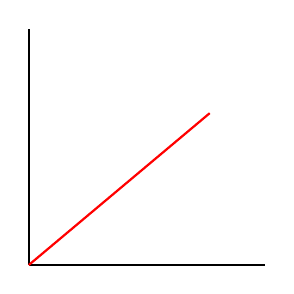
\begin{tikzpicture}
\draw [thick] ( 0,0) -- (3,0);
\draw [thick] ( 0,0) -- (0,3);
\draw [red,thick] ( 0,0) -- (400:3);
\bigangle[blue,dashed]{400}
\end{tikzpicture}
\end{document}
\end{verbatim}

% \includegraphics{https://i.stack.imgur.com/4RO8Y.png}{图片图片}


\faq{如何画交换图?}{}


\faq{如何在插入的图(\cs{includegraphics}\Arg{...})的特定位置插入符号或图}{}

可以使用 overpic 宏包,在 overpic 环境内进行图形绘制,环境内可以使用
latex 自生 picture 环境的绘图语句进行绘制。以下面给出一个例子:

\begin{verbatim}
\documentclass{article}
\usepackage{graphicx}
\usepackage{overpic}
\begin{document}
\begin{overpic}[width=0.8\textwidth
               %,grid,tics=10 % 取消注释可以产生网格线帮助定位,完成后再将其注释。
               ]{1.png}
  \put(35,10){\LaTeX}
  \put(80,0){\includegraphics[width=0.16\textwidth]{1.png}}
\end{overpic}
\end{document}
\end{verbatim}

下面左边是原图,右边是代码处理后的图片:
% \includegraphics{https://images-cdn.shimo.im/VFe2jSxjmoMZpr2B/1.png!thumbnail}
% \includegraphics{https://images-cdn.shimo.im/4qswwF2P4u44JNYB/2.png!thumbnail}

当然还有一种方法可以使用 tikz 宏包,在 tikzpicture
环境引入图片,并在此基础上进行绘图,这样的优点是绘图语句更为丰富,功能更强大。下面举个例子:

\begin{verbatim}
       ![图片](https://images-cdn.shimo.im/LrJDsfrVZIAerfPW/image.png!thumbnail)  ![图片](https://images-cdn.shimo.im/sVlNCmljor0SctYs/image.png!thumbnail)
\end{verbatim}

第一个为原图,第二个是在原图基础上添加一个标号和边.
其中的格线是用来辅助做图的。

\begin{verbatim}
\documentclass{article}
\usepackage{tikz}
\begin{document}
\pgfdeclarelayer{foreground}
\pgfdeclarelayer{background}
\pgfsetlayers{background,main,foreground}
\begin{tikzpicture}
\begin{pgfonlayer}{background}
\path[xshift=-1.24pt,yshift=4pt]      (0,0) node (o) {
  \includegraphics[width=2.8cm]{graph.pdf}};
\end{pgfonlayer}
\begin{pgfonlayer}{foreground}
    \node at (0,0) [label={[label distance=-2mm]40:$u$}]{};
    \draw[step=.5cm,help lines] (-1.4,-1.4) grid (1.4,1.4);
    \coordinate (A) at (0,1.36);
    \coordinate (B) at (0.91,-1.14);
    \fill[color=red] (B) circle (1pt);
    \draw[line width=0.6pt](A)--(B);
\end{pgfonlayer}
\end{tikzpicture}
\end{document}
\end{verbatim}

% % Copyright (C) 2018 by latexstudio <http://www.latexstudio.net>
%
% This program is free software: you can redistribute it and/or modify
% it under the terms of the GNU General Public License as published by
% the Free Software Foundation, either version 3 of the License, or
% (at your option) any later version.
%
% This program is distributed in the hope that it will be useful,
% but WITHOUT ANY WARRANTY; without even the implied warranty of
% MERCHANTABILITY or FITNESS FOR A PARTICULAR PURPOSE.  See the
% GNU General Public License for more details.
%
% You should have received a copy of the GNU General Public License
% along with this program.  If not, see <http://www.gnu.org/licenses/>.
%

\section{开发篇(含 \LaTeX3)}
%
%介绍宏开发技巧,宏包和模板类开发的常见问题。
%\end{faq}
%
%
%\begin{faq}{在阅读已有的宏包或者文类时,遇到未知的命令应如何处理}
%
%可以参照胡伟的《LaTeX2e文类和宏包学习手册》中的第四章-命令集注。
%
%
%

% % Copyright (C) 2018 by latexstudio <http://www.latexstudio.net>
%
% This program is free software: you can redistribute it and/or modify
% it under the terms of the GNU General Public License as published by
% the Free Software Foundation, either version 3 of the License, or
% (at your option) any later version.
%
% This program is distributed in the hope that it will be useful,
% but WITHOUT ANY WARRANTY; without even the implied warranty of
% MERCHANTABILITY or FITNESS FOR A PARTICULAR PURPOSE.  See the
% GNU General Public License for more details.
%
% You should have received a copy of the GNU General Public License
% along with this program.  If not, see <http://www.gnu.org/licenses/>.
%

\section{常见错误提示}
%
%\begin{itemize}
%  \item
%  ! LaTeX Error: File `xxx.sty' not found.
%  \cs{usepackage}时,引用错误宏包名称或者本机未下载相应的宏包。解决方法为检查拼写,或TeXLive使用tlmgr安装宏包。
%  \item
%  ! LaTeX Error: File `xxx.cls' not found.
%  \cs{documentclass}时,引用错误文类名称或者本机未下载相应的文类。解决方法为检查拼写,或TeXLive使用tlmgr安装文类。
%  \item
%  ! Undefined control sequence.
%  编译遇到不存在的命令(未定义的控制序列)。解决方法为检查拼写,引用相应的宏包,或者定义该命令。
%  \item
%  ! Missing \{ inserted. 或者 ! Missing \} inserted.
%  缺少分组的某个花括号。解决方法为仔细查找上下文对应的花括号。
%  \item
%  ! Missing \$ inserted.
%  缺少数学环境,通常为把数学环境专用的命令用在普通文本模式。
%  \item
%  ! LaTeX Error: Can be used only in preamble.
%  有许多命令只能用于导言区,如果在document
%  环境中用了这些命令,将显示上面的错误信息。
%  \item
%  ! LaTeX Error: Counter too large.
%  计数器数值太大,一般是在需要以字母形式显示的计数器其数值超过了26。
%  \item
%  ! LaTeX Error: \cs{include} cannot be nested.
%  在一个已经要用 \cs{include} 引入的文件中又使用了
%  \cs{include} 命令。
%  \item
%  ! LaTeX Error: Missing \verb|\begin{document}|
%  这种情况可能是忘了输入 \verb|\begin{document}|,或者是在导言区中有可打印的文本,还有可能是编译中断时在
%  aux 等辅助文件中写入错误,对于后者,可以清理辅助文件后重新进行编译。
%  \item
%  ! LaTeX Error: No counter `xxx' defined.
%  调用某计数器,但该计数器并不存在。
%  \item
%  ! LaTeX Error: No \cs{title} given. 在给出
%  \cs{title} 声明之前就使用了 \cs{maketitle} 命令。
%  \item
%  ! LaTeX Error: Something's wrong--perhaps a missing \cs{item}.
%  导致这个问题一般是在列表环境中的文本不是由 \cs{item} 开始的。
%  \item
%  ! LaTeX Error: There's no line here to end.
%  在 \cs{par} 或空行后调用命令 \cs{newline} 或 \verb|\\|。
%  这里它们没有任何意义,如果需要额外竖直间距,应使用 \cs{vspace} 命令。
%  \item
%  ! LaTeX Error: Lonely \cs{item} -- perhaps a missing list enviroment.
%  在列表环境外使用了 \cs{item} 命令。
%\end{itemize}
%\end{faq}
%
%
%


\end{document}


\documentclass{article}
\usepackage{fontspec}
\begin{document}
\IfFontExistsTF{SourceHanSerif.ttc}{SourceHanSerif True}{SourceHanSerif False}
\IfFontExistsTF{SourceHanSerif-Regular.ttc}{SourceHanSerif-Regular True}{SourceHanSerif-Regular False}
\end{document}
